\chapter{Introduction to Causal Effect}

\section{Causal effect}
\noindent {\bfseries Outline:}\\
1. Two types of causal effect: "average causal effect" and 
"the causal effect of treatment on the treated".\\
2. The difference between conditioning and variables versus setting(manipulating) variables.
\subsection{The definition of "Average Causal Effect"}
在上帝的hypothetical worlds中,population of interest是某个感兴趣的目标群体. In hypothetical world 1,population中的每个人都接受处理$A=0$,对应的outcome记为$Y^0$;  In hypothetical world 2,the same population 全部接受另一种处理$A=1$,对应的outcome记为$Y^1$. 如果可以同时观测到这两个worlds的outcome data,那么average causal effect为
\begin{equation}
\setlength{\abovedisplayskip}{3pt}
\setlength{\belowdisplayskip}{3pt}
\label{ace}
ACE=E(Y^1 -Y^0)
\end{equation}
公式(\ref{ace})是用average value of Y if everyone was treated with $A=1$ 减去 the average value of Y if everyone was treated with $A=0$. 通过Fig.\ref{ACE}更容易理解.
\begin{figure}[htbp]
	\setlength{\abovecaptionskip}{0pt}     %调整图片标题与图距离
	\setlength{\belowcaptionskip}{0pt}
	\vspace{-0cm}  %调整图片与上文的垂直距离
	\setlength{\abovecaptionskip}{-0cm}   %调整图片标题与图距离
	\setlength{\belowcaptionskip}{0cm}   %调整图片标题与下文距离
	\centering
	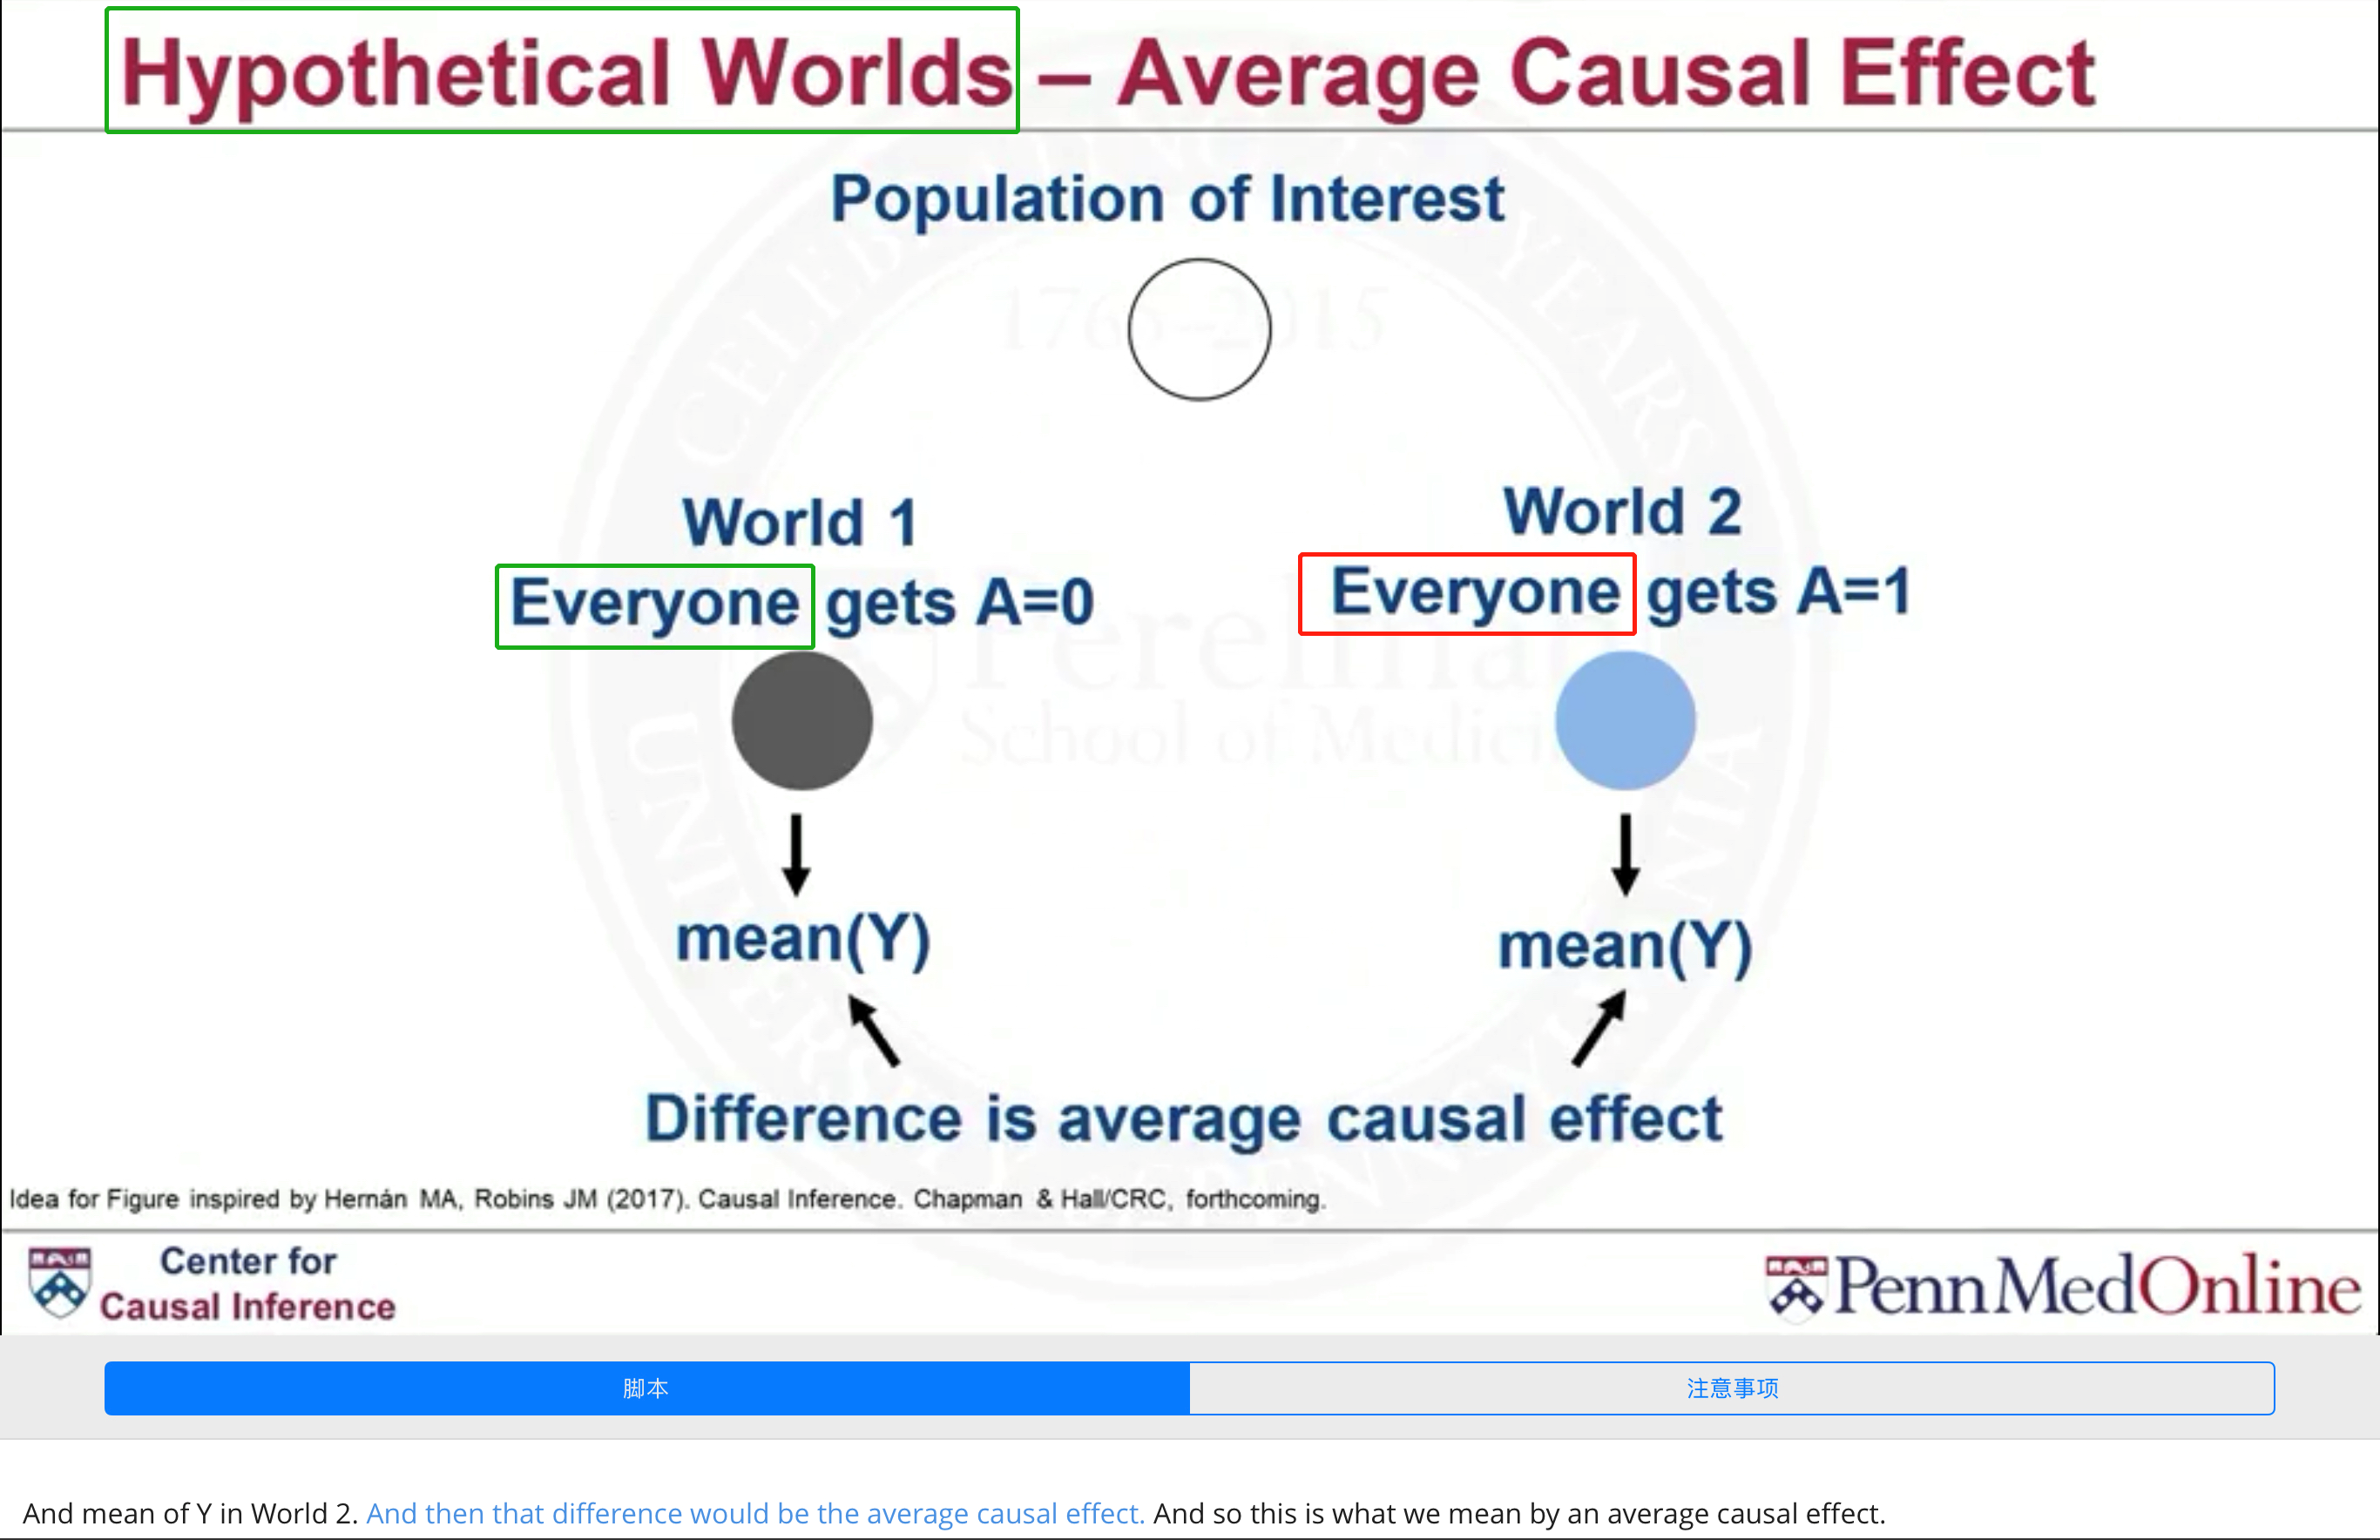
\includegraphics[width=0.7\textwidth]{figure/ACE.png}
	\caption{Average Causal Effect}
	\label{ACE}
\end{figure}

\subsection{Conditioning on versus setting}
这一部分主要是辨析概念:
\begin{equation}
E(Y^1-Y^0) \neq E[Y|A=1]- E[Y|A=0]
\end{equation}
\begin{itemize}[itemindent = 0em]
    \item[$\blacktriangleright$]$E(Y^1-Y^0)$是whole population都进行处理$A=1$与whole population都进行处理$A=0$时average outcome的差值. 
    \item[$\blacktriangleright$]$E[Y|A=a]$是在给定$A=a$的情况下$Y$的均值,相当于在$A=a$的这部分人中求average outcome. 于是$E[Y|A=1]-E[Y|A=0]$表示$A=1$的这部分人与$A=0$的另一部分人的average outcome的差值.
\end{itemize}

对象从population变成了subpopulation. 所以两者本质是不一样的:
\begin{itemize}[itemindent = 2em]
	\item Setting(manipulating) treatment $\Longrightarrow$ potential outcome situation.
    \item Conditioning on $\Longrightarrow$ restricting to subpopulation.
\end{itemize}

slides如Fig.\ref{versus}所示.
\begin{figure}[htbp]
	\setlength{\abovecaptionskip}{0pt}     %调整图片标题与图距离
	\setlength{\belowcaptionskip}{10pt}
	\vspace{-0cm}  %调整图片与上文的垂直距离
	\setlength{\abovecaptionskip}{-0cm}   %调整图片标题与图距离
	\setlength{\belowcaptionskip}{0cm}   %调整图片标题与下文距离
	\centering
	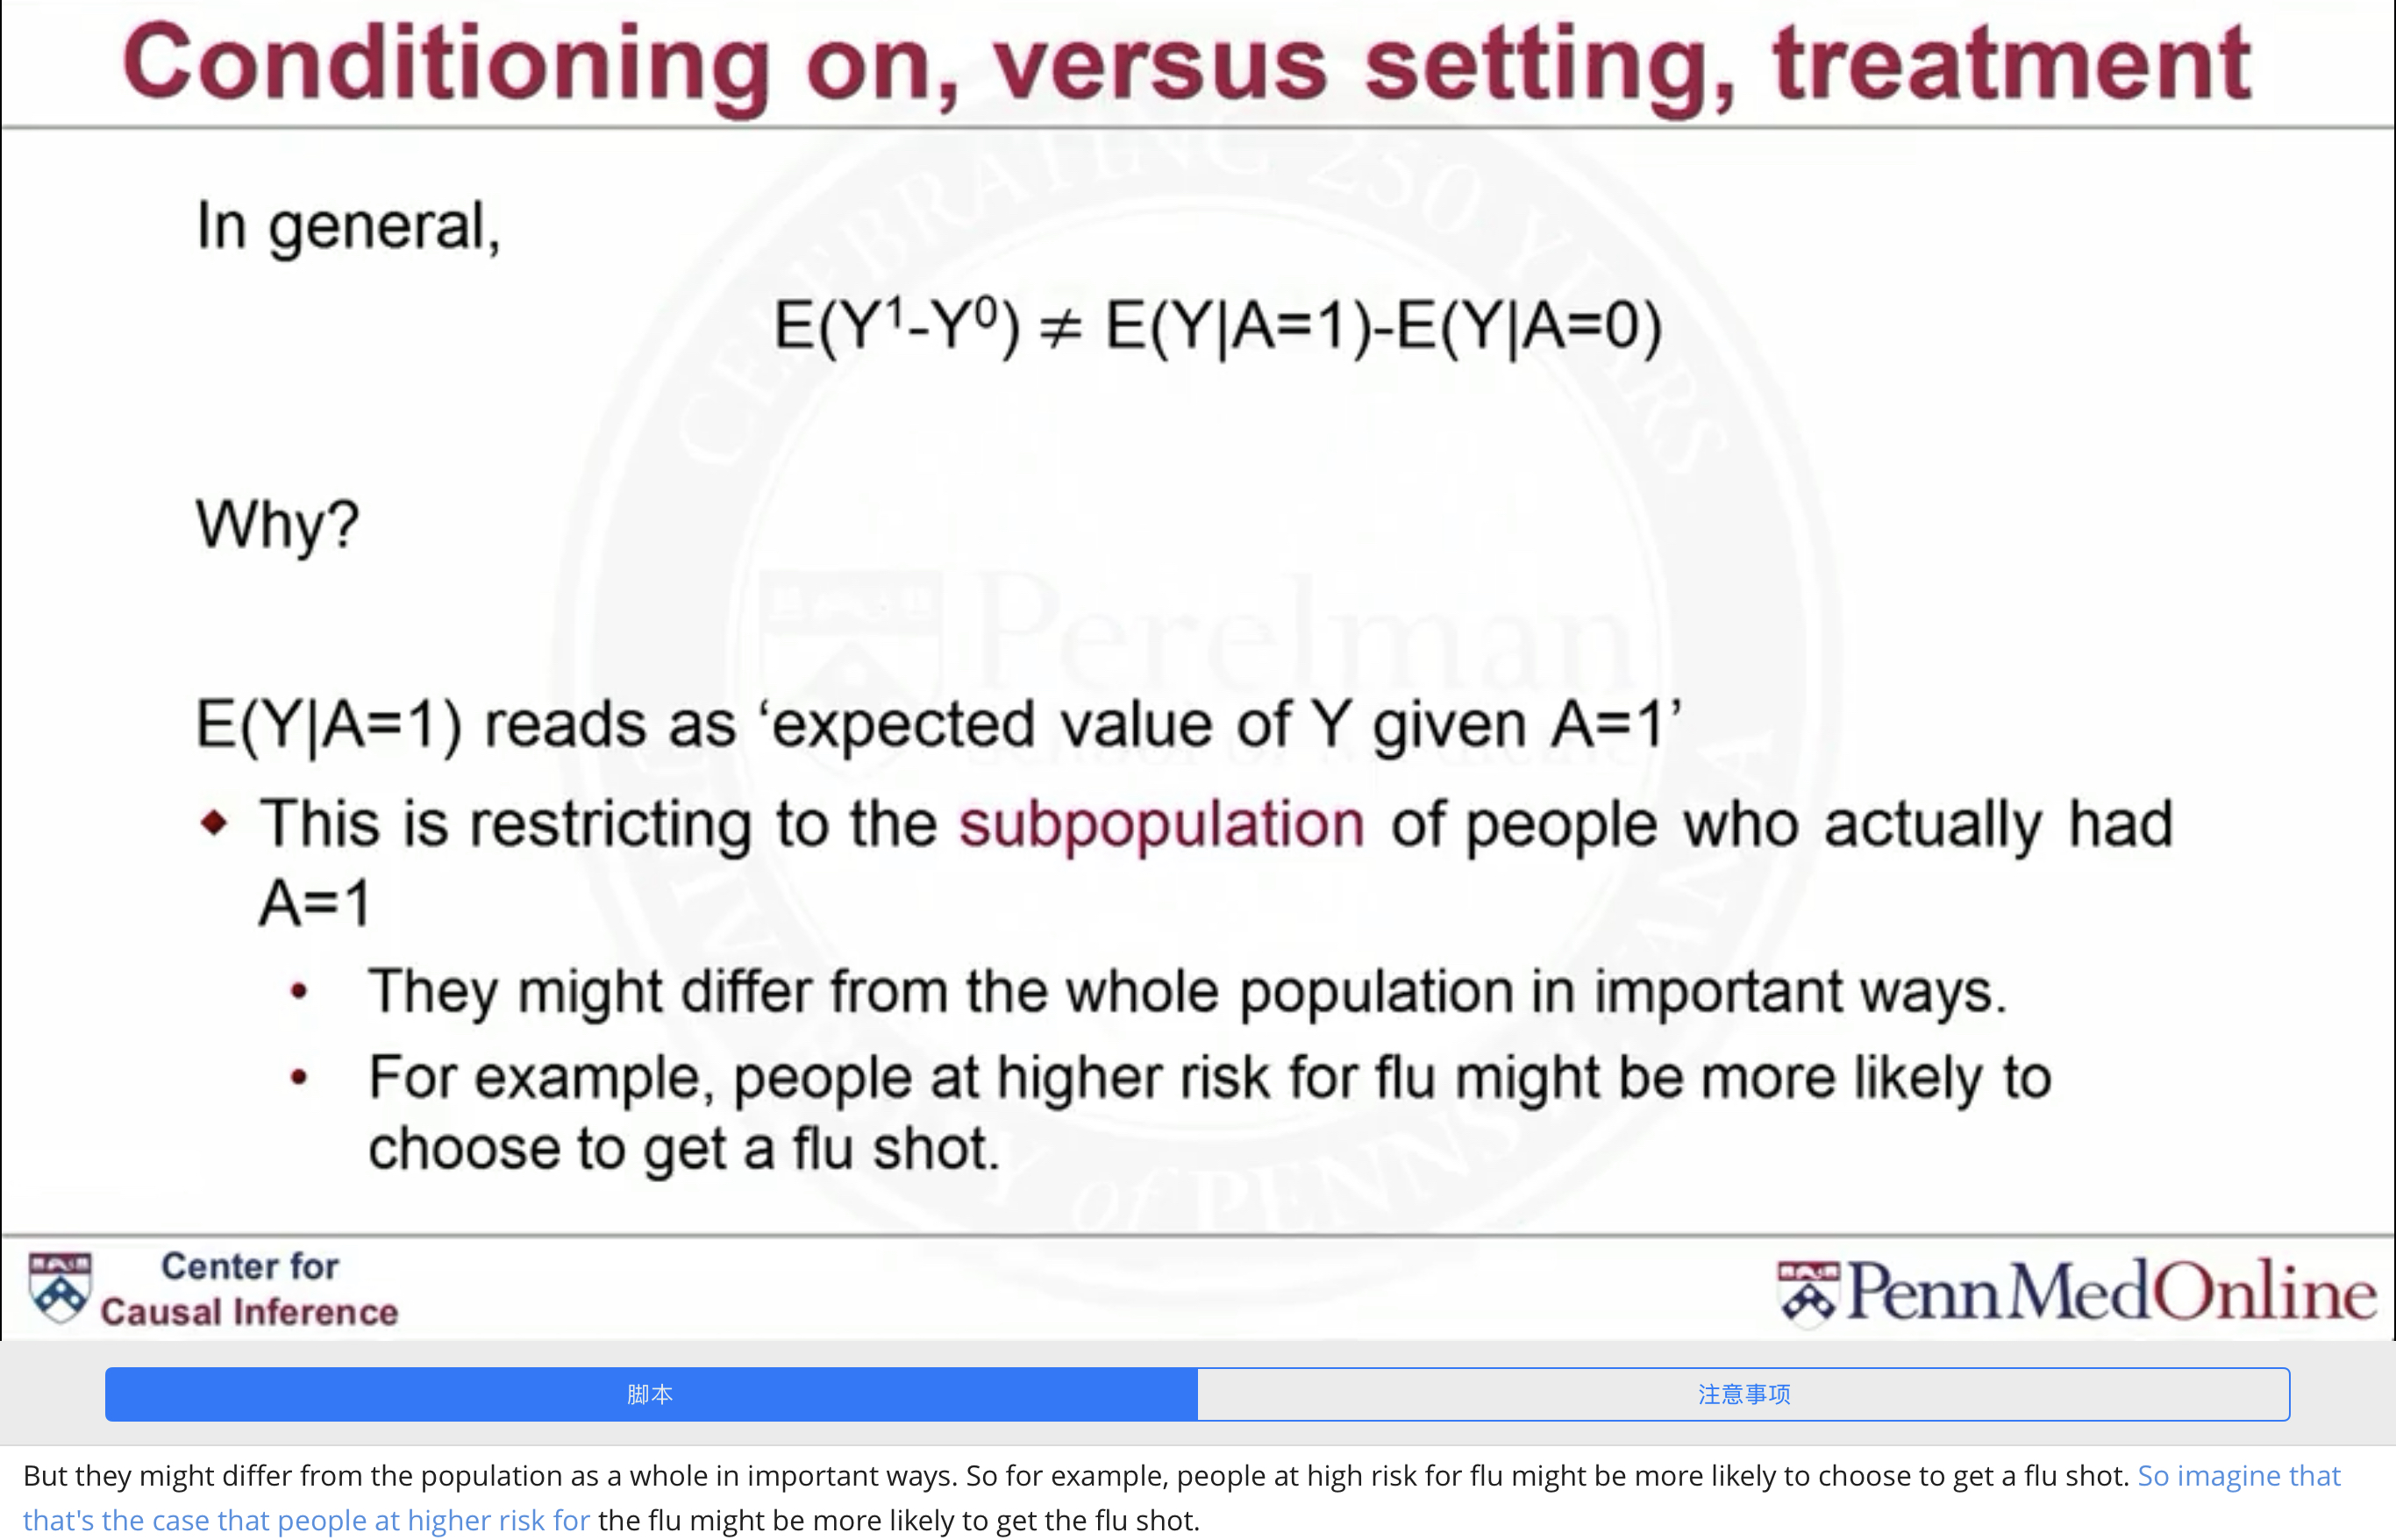
\includegraphics[width=0.8\textwidth]{figure/versus.jpg}
	\caption{Conditioning on,versus setting,treatment}
	\label{versus}
\end{figure}
	
\subsection{The definition of "the causal effect of treatment on the treated"}
这个概念是针对subpopulation来说的. 直接看slides就能明白,如Fig.\ref{CETT}.
\begin{figure}[htbp]
	\setlength{\abovecaptionskip}{0pt}     %调整图片标题与图距离
	\setlength{\belowcaptionskip}{10pt}
	\vspace{-0cm}  %调整图片与上文的垂直距离
	\setlength{\abovecaptionskip}{-0cm}   %调整图片标题与图距离
	\setlength{\belowcaptionskip}{-0cm}   %调整图片标题与下文距离
	\centering
	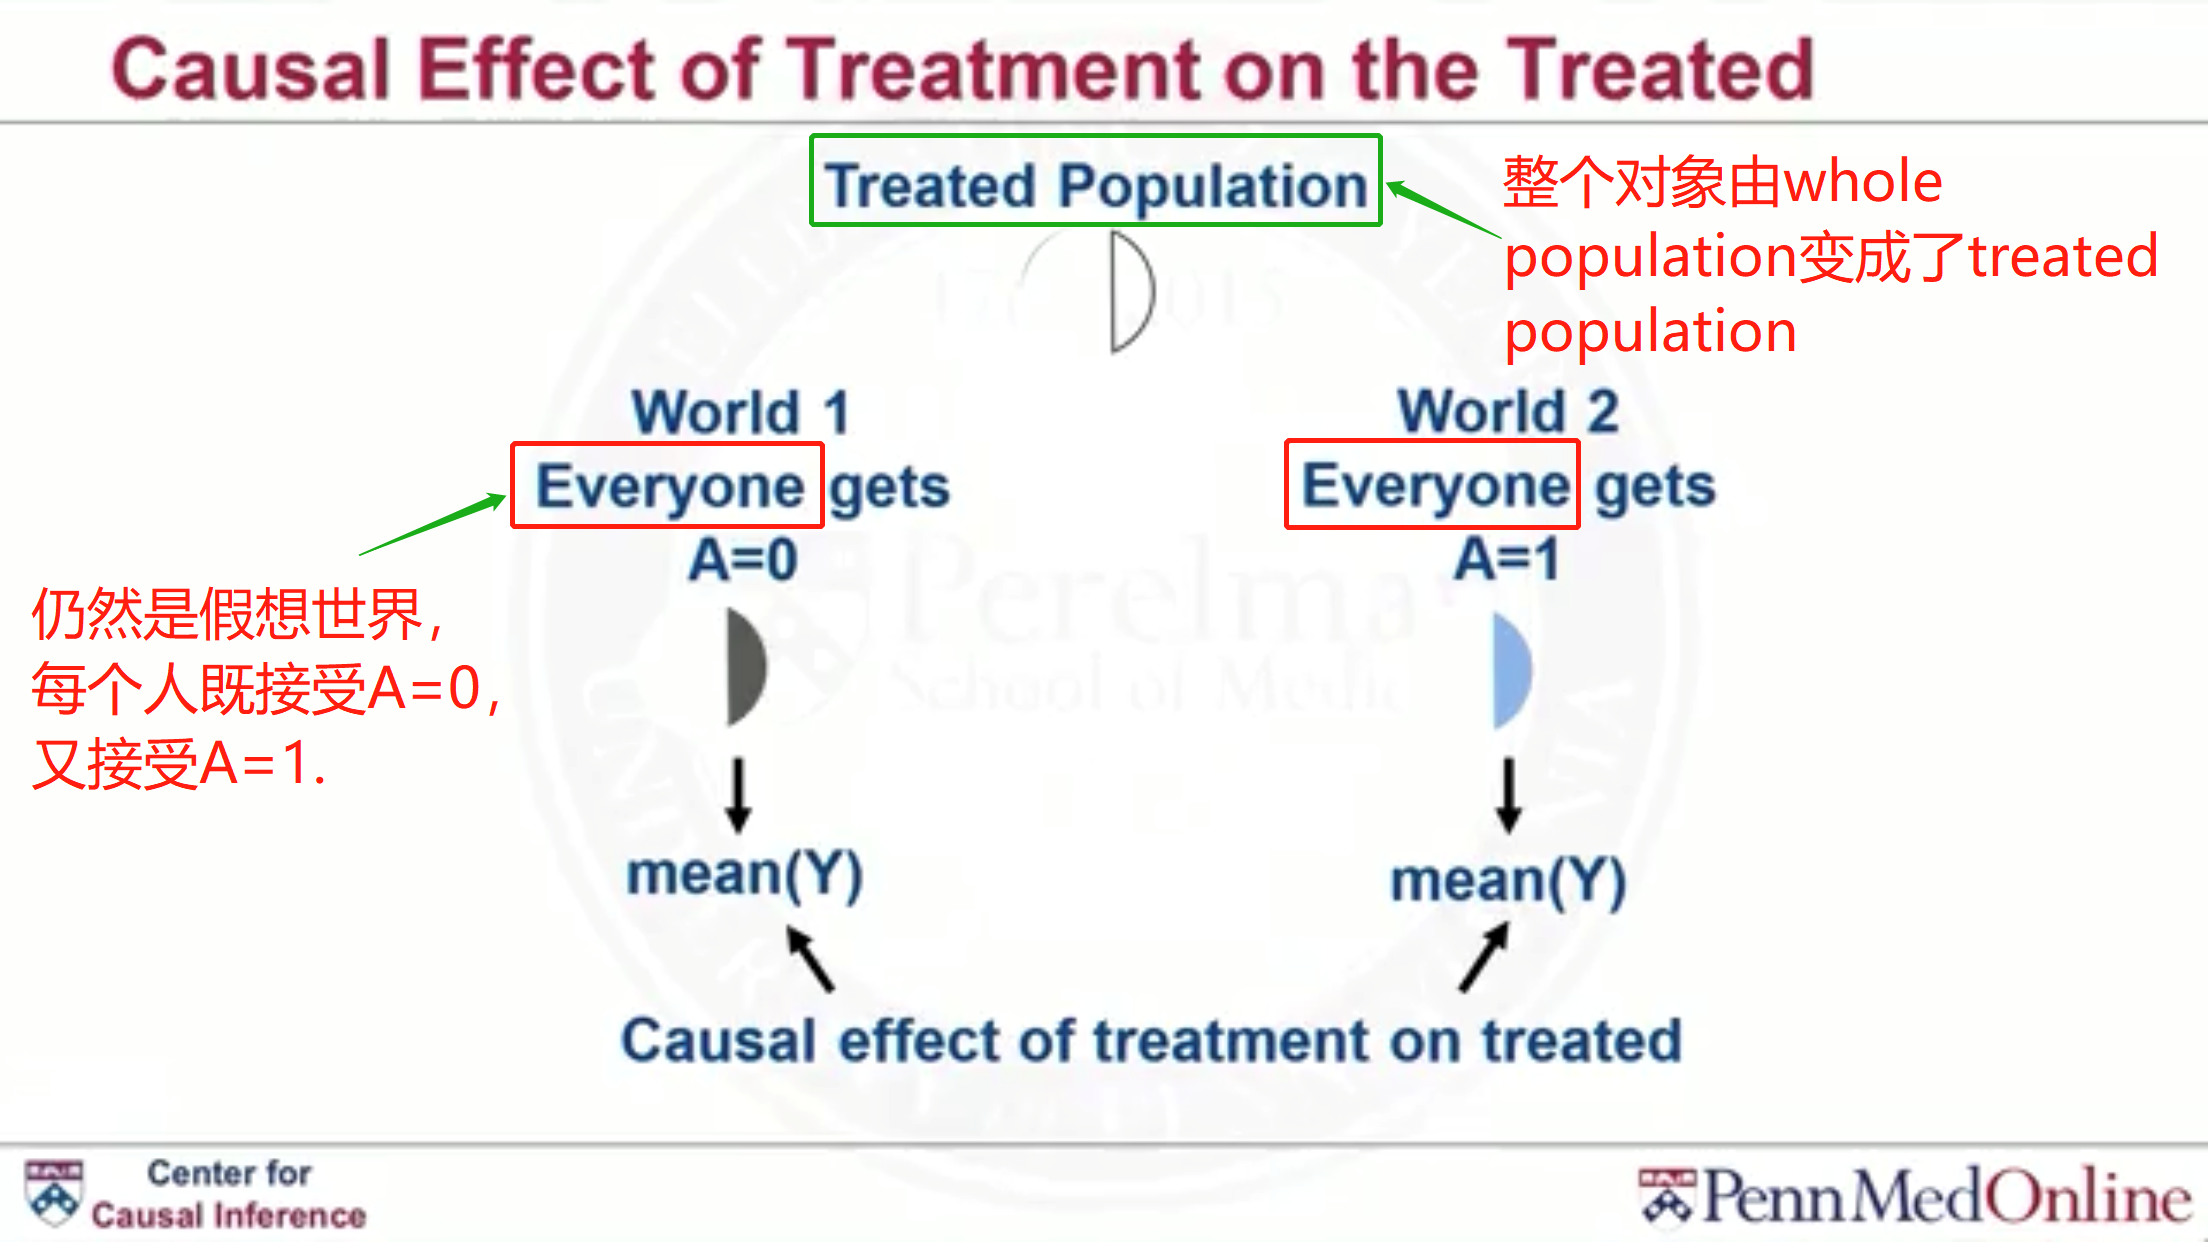
\includegraphics[width=0.8\textwidth]{figure/CETT.png}
	\caption{The causal effect of treatment on the treated}
	\label{CETT}
\end{figure}

\subsection{Conclusion}
从这一课中我们学到了非常重要的概念辨析. 什么是causal effect?为什么条件均值差$E[Y|A=1]-E[Y|A=0]$不能作为causal effect?
这些概念的重点在于区分{\color{red}treatment是针对whole population还是whole population中的不同subpopulation. }
Causal effect之所以是Causal effect,是因为它针对的是整个population的潜在结果差异. 现实中不可度量. 而其他条件均值差之所以不能作为Causal effect,是因为它针对的是different people的结果差异.
这一点非常重要. 以一张图可以总结这一课的重点:
\begin{figure}[htbp]
	\setlength{\abovecaptionskip}{0pt}     %调整图片标题与图距离
	\setlength{\belowcaptionskip}{10pt}
	\vspace{-0cm}  %调整图片与上文的垂直距离
	\setlength{\abovecaptionskip}{-0cm}   %调整图片标题与图距离
	\setlength{\belowcaptionskip}{-0cm}   %调整图片标题与下文距离
	\centering
	\includegraphics[width=0.8\textwidth]{figure/ConditionVSsetting.png}
	\caption{Conditioning Versus setting}
	\label{ConditionVSsetting}
\end{figure}

% 第一章新课时 
\newpage \section{Causal Assumptions} \label{Causal assumption}
\noindent {\bfseries Outline}:
\begin{itemize}
	\item[$\blacktriangleright$] Identifiability
	\item[$\blacktriangleright$] SUTVE 
	\item[$\blacktriangleright$] Consistency assumption
    \item[$\blacktriangleright$] Ignorability assumption
    \item[$\blacktriangleright$] Positivity assumption
\end{itemize}

\subsection{Identifiability}
Statistical identifiability: If a parameter can be estimated from actual data, it is considered identifiable.

{\color{red} Identifiability of causal effect} requires making some {\color{red} untestable} assumptions.
Assumptions will be about the observed data:$Y,A,X$.
假设是为了让我们能够从观测数据中识别Causal effect,因为实际上causal effect是不可观测的,所以估计causal effect需要加一些假设. 
\subsection{Stable Unit Treatment Value Assumption}
SUTVA的含义分为两层,No inference and one version of treatment.\\
\noindent (1) {\color{red} No inference:}
\begin{enumerate}[labelindent=2\parindent, leftmargin=*,align=left,widest=IV,label=\Roman*.]
	\item 每个受试者之间没有相互影响.
	\item 一个受试者的处理分配不会影响其他受试者的outcome. 
\end{enumerate}

这意味着每个受试者的outcome与其他人是无关的.\\

\noindent(2) {\color{red} One version of treatment:}

There is one variable that we can hypothetically intervene on and it's very well defined what we mean by treatment.
这一部分的作用是使得treatment的意义更加明确,假设我们干预了某个variale,并且这个variable就是我们定义的treatment.

SUTVA的作用就是“我们可以把第$i$个受试者的potential outcome” 表示成其自身所接受的treatment的形式. 而不受其他受试者的影响.

\subsection{Consistency Assumption}
The potential outcome under treatment $A=a: Y^a$ is equal to the observed outcome $Y$ if the actual treatment received is $A=a$.
\begin{equation}
\text{observed outcome  }Y = Y^a,\quad \text{if A=a, for all a.}
\end{equation} 
这则假设告诉我们,真实处理$A=a$下的观测结果$Y$可以看做接受处理$A=a$时的potential outcome.

\subsection{Ignorability assumption}
Given pre-treatment covariates $X$, treatment assignment is independent from the potential outcomes. Or Potential outcomes are independent of treatment assignment conditional on covariates X.
\begin{equation}
Y^0,Y^1 \perp A|X.
\end{equation}
这则假设说明在给定$X$后,对于$X$取值相同的受试者来说,处理$A$的分配是随机的. Potential outcome与处理的分配无关. 

此外,Ignorability assumption还有两个别称:
\begin{enumerate}[label=(\arabic*)]
	\item Conditional independence assumption(CIA):Conditioning on $X$,$Y^0, Y^1$与$A$独立. 
    \item No unmeasured confounders, 指所有的confounders都被measure到,控制了这些confounders就可以把$A$看做是随机分配的.
\end{enumerate}


\subsection{Positivity Assumption}
For every set of values for $X$, treatment assignment was not deterministic:
\begin{equation}
P(A=a|X=x)>0,\text{  for all a and x.}
\end{equation} 

这则假设说明:对于给定的$X$,每个个体都有可能接受任何处理. 如果某个个体不可能接受another treatment,也就意味着我们不能观测到他的potential outcome. 这就违背了causal effect的本质.

\subsection{Observed Data and Potential Outcomes}
结合上述4条假设,是通过observed data识别causal effect的基础. 实现从$E(Y|A=a,X=x)$到$E(Y^a|X=x)$的转化. Fig.\ref{assump}很好地说明了assumptions在因果推断中的作用.
\begin{figure}[htbp]
	\setlength{\abovecaptionskip}{0pt}     %调整图片标题与图距离
	\setlength{\belowcaptionskip}{10pt}
	\vspace{-0cm}  %调整图片与上文的垂直距离
	\setlength{\abovecaptionskip}{-0cm}   %调整图片标题与图距离
	\setlength{\belowcaptionskip}{-0cm}   %调整图片标题与下文距离
	\centering
	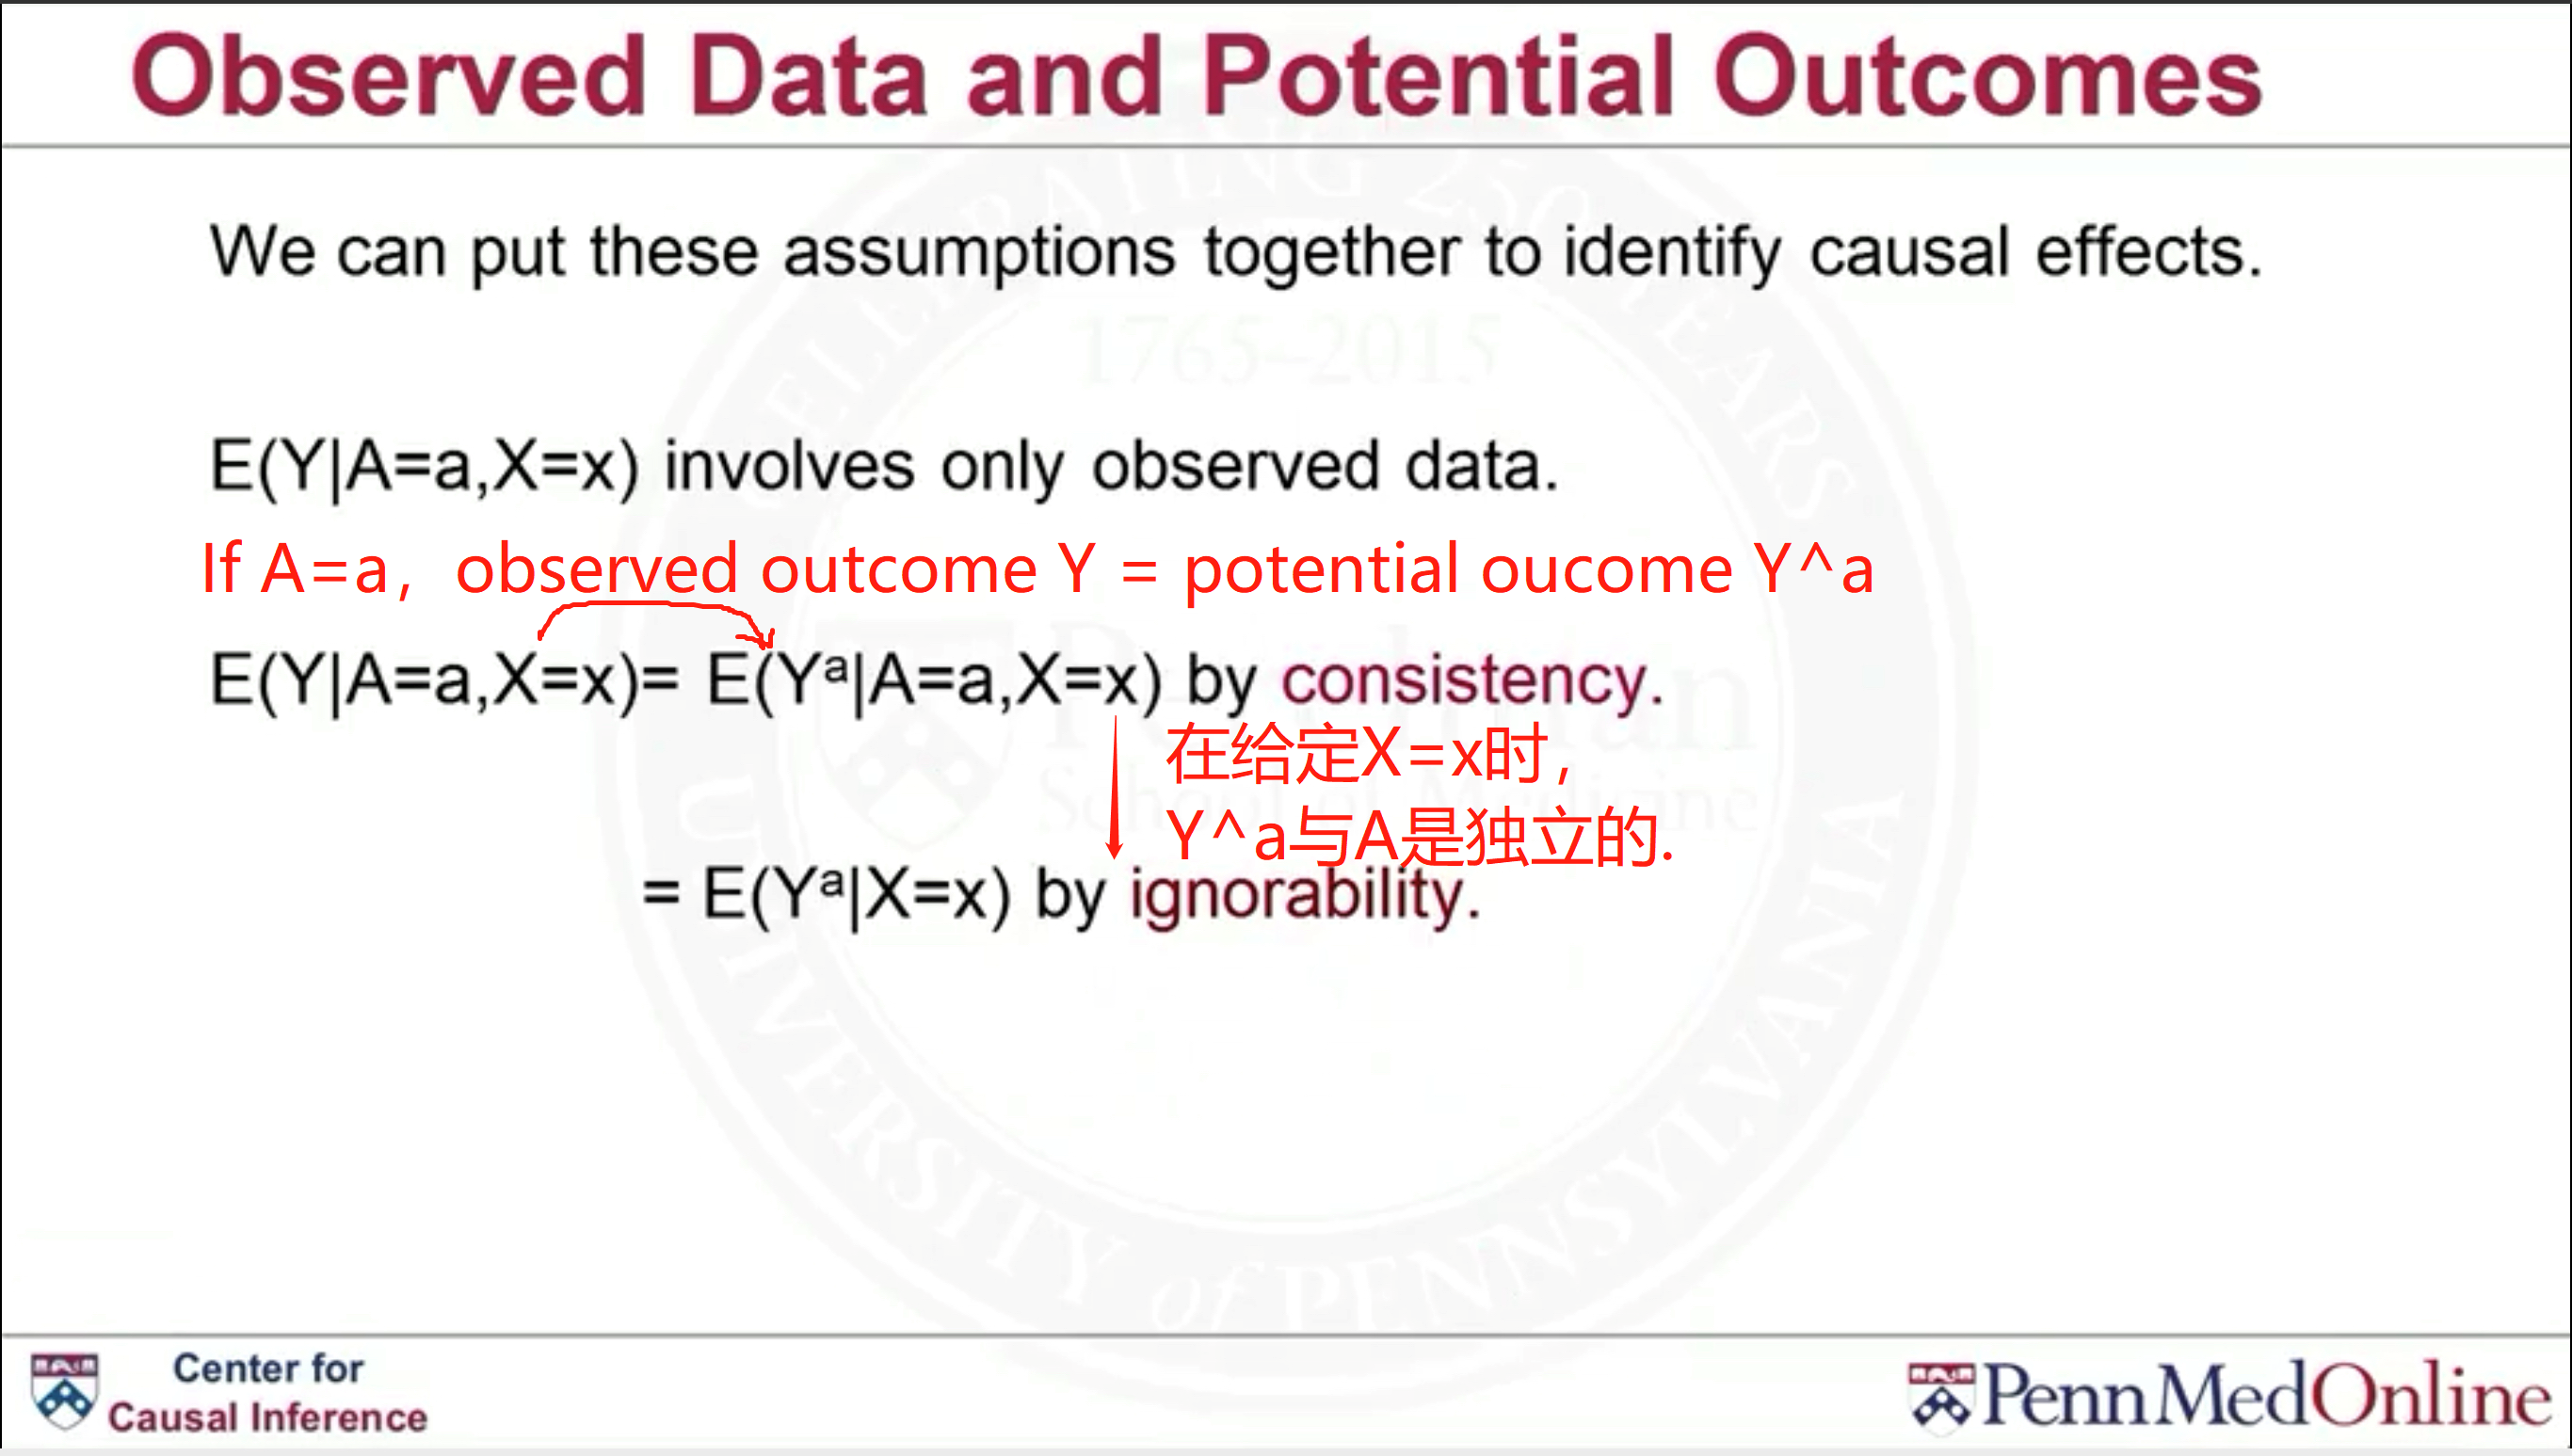
\includegraphics[width=0.8\textwidth]{figure/assump.png}
	\caption{Observed Data and Potential Outcomes}
	\label{assump}
\end{figure}

\newpage \section{Stratification}
这一部分讲了估计causal effect的一种简单思想,但只适用于非常简单的情形,因此几乎没有实际应用.

在第\ref{Causal assumption}节中,我们已经知道通过假设可以实现
\begin{equation}
E(Y|A=a,X=x)=E(Y^a|X=x)
\end{equation}
那么potential outcome的均值就可以通过遍历$X$的取值求得:
\begin{equation}
E(Y^a)=\sum_{x} E(Y^a|X=x)P(X=x) =\sum_{x} E(Y|A=a,X=x)P(X=x)
\end{equation}
称$E(Y^a)$为standardized mean. 

Standardization包含了"stratifying"和"averaging"两层结构.
我们可以将所有样本按照$X$和$A$分层,然后分别求出在不同的$X$和$A$下outcome的均值.下面用一个例子说明Stratification的用法. 
\begin{ex}
某机构正在研究两种药物:saxagliptin(简称saxa)和sitagliptin(简称sita)对主流心脏病发病(MACE)的影响. 口服抗糖尿病药物(oral antidiabetic drug,简称OAD)是协变量. 已知选择药物saxagliptin治疗的病人之前多服用过OAD,而服用OAD的病人有更高的患MACE的风险.
\end{ex}

现在我们整理一下解题思路:\\
\begin{figure}[htbp]
	\setlength{\abovecaptionskip}{0pt}     %调整图片标题与图距离
	\setlength{\belowcaptionskip}{10pt}
	\vspace{-0cm}  %调整图片与上文的垂直距离
	\setlength{\abovecaptionskip}{-0cm}   %调整图片标题与图距离
	\setlength{\belowcaptionskip}{-0cm}   %调整图片标题与下文距离
	\centering
	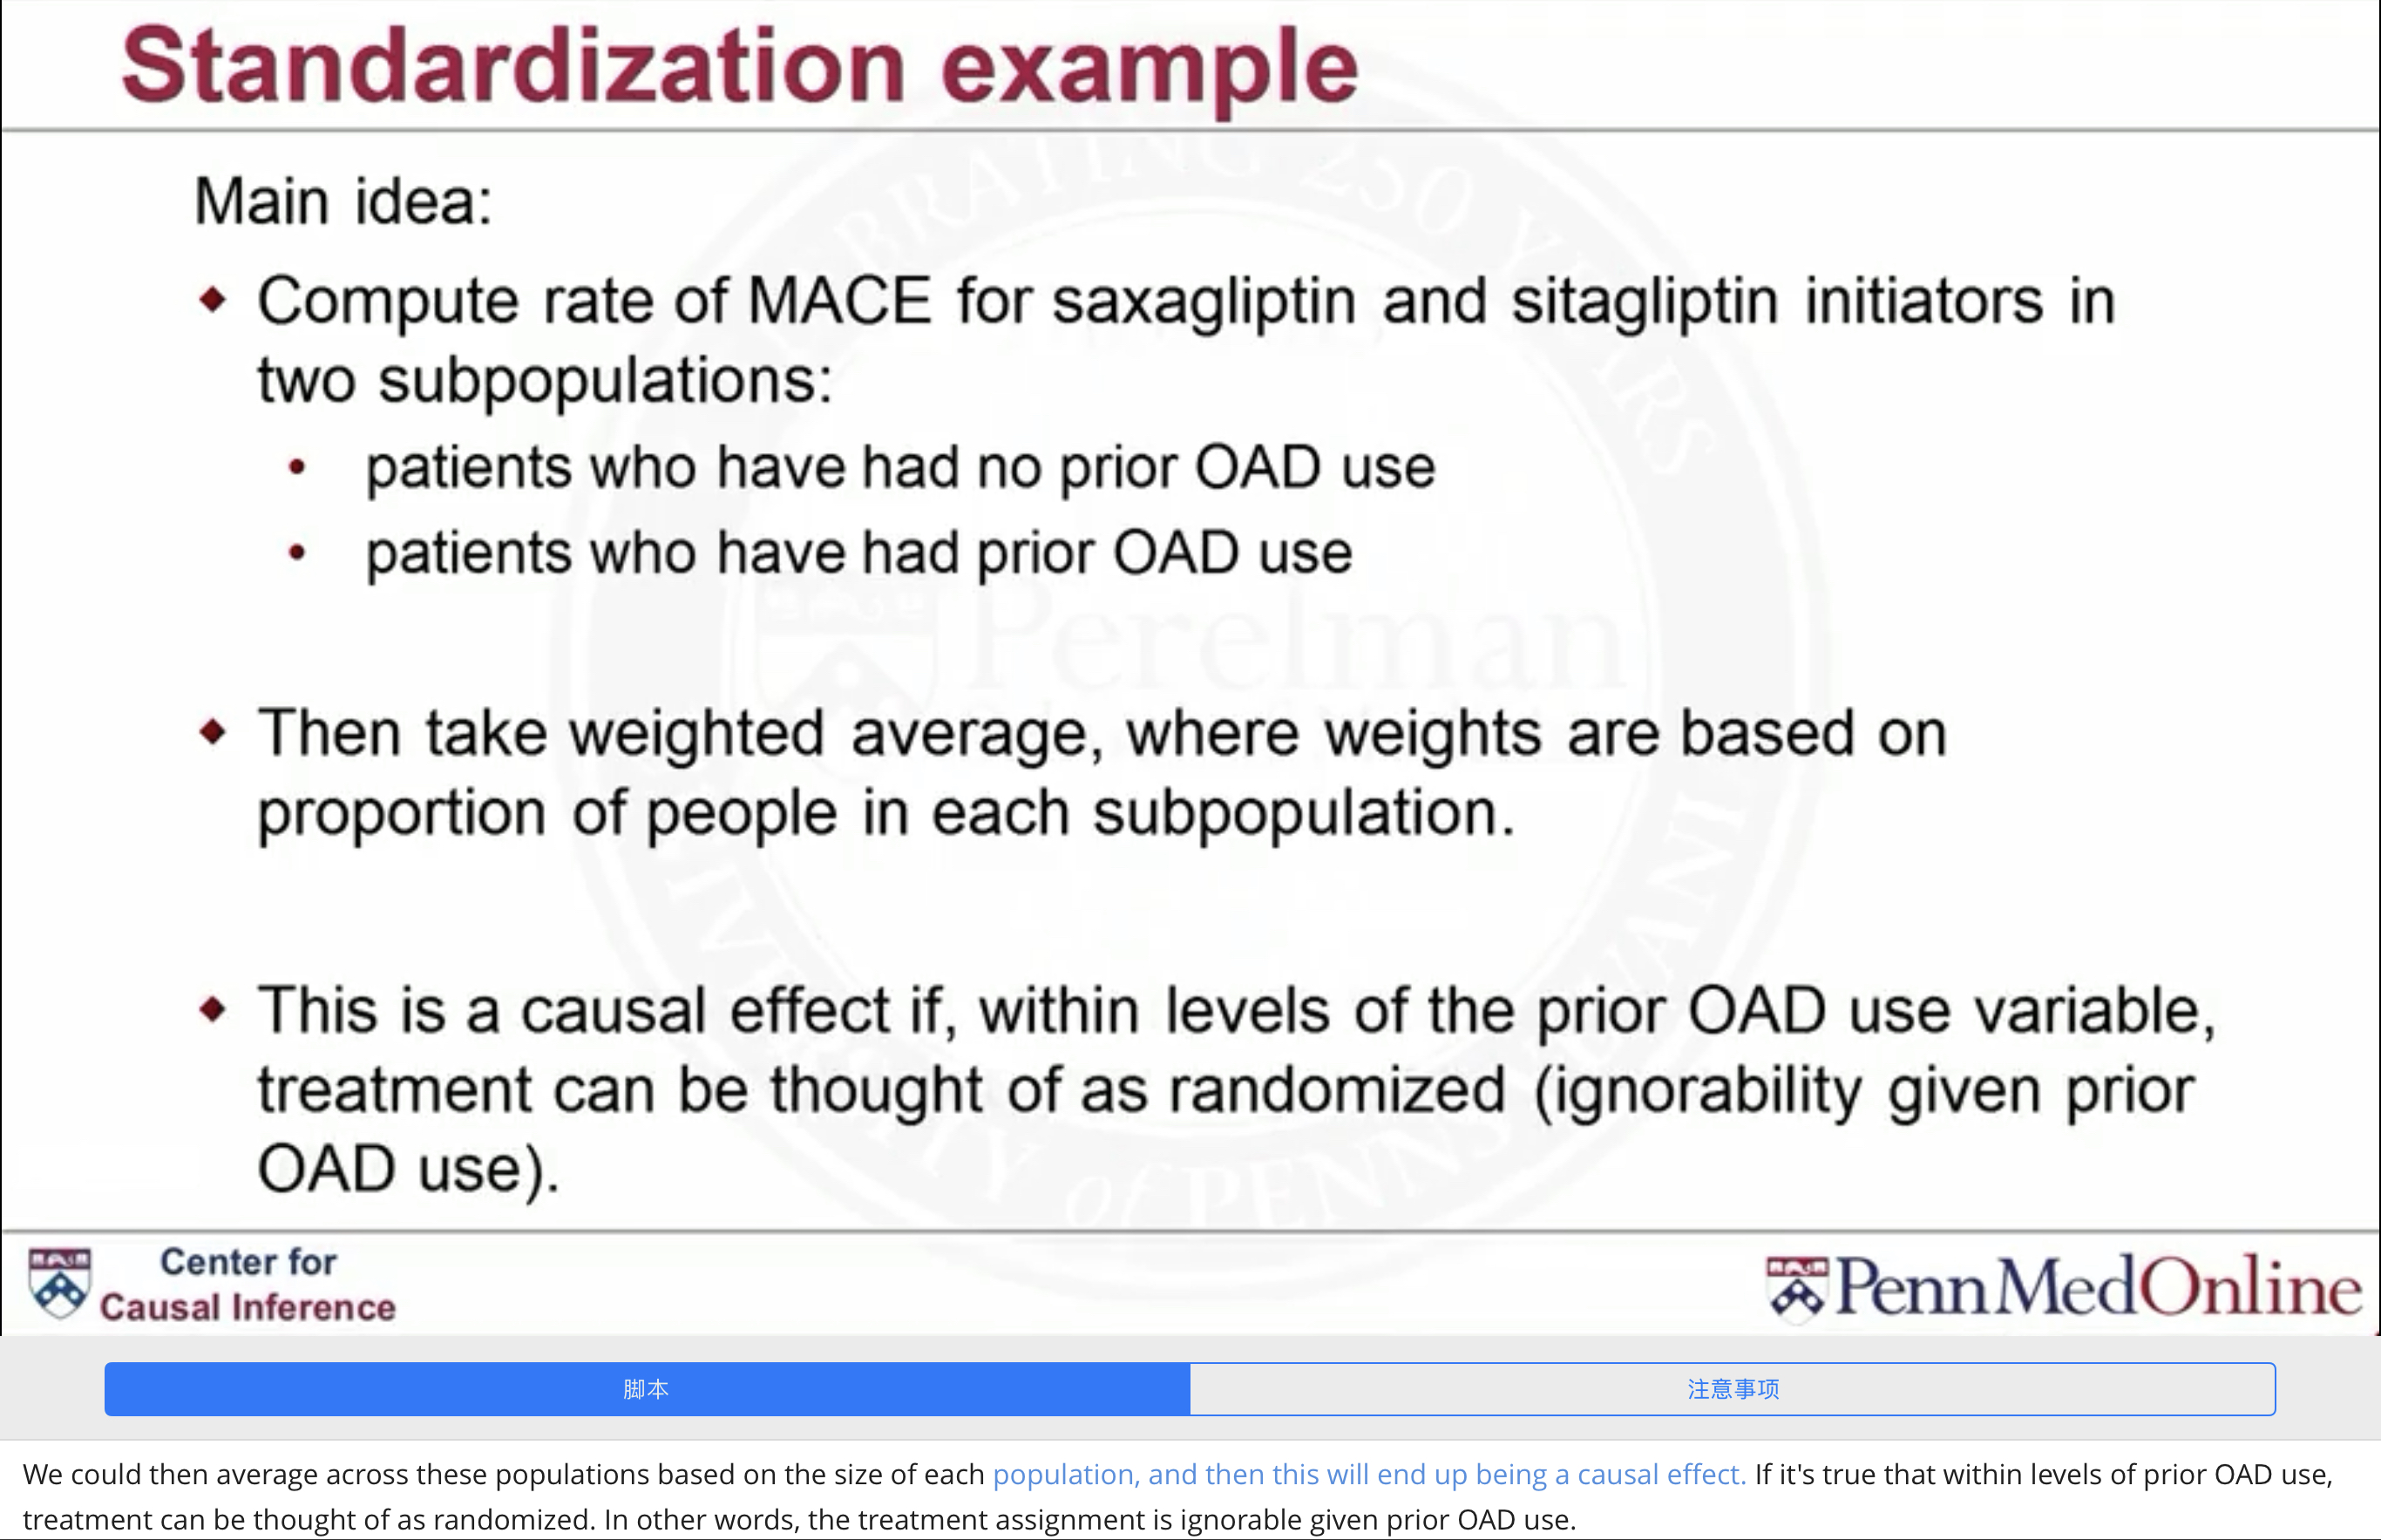
\includegraphics[width=0.8\textwidth]{figure/strtidea.jpg}
	\caption{Main idea of Stratification}
	\label{strtidea}
\end{figure}

接下来要做的就是按照$X$将数据分层:服用过OAD的分为一组,在whole population中所占的比例记为P(prior OAD use yes);未服用过OAD的分成另一组,所占比例记为P(prior OAD use no). 

在每一组中再按照$A$的取值划分层次:$A=saxa$划为一层,$A=sita$的划为另一层. 共得到4层样本,然后在每一层上计算患MACE的比例. 计算的过程如Fig.\ref{meansaxa}和Fig.\ref{meansita}所示.
    \begin{figure}[htbp]
	%\setlength{\abovecaptionskip}{0pt}     %调整图片标题与图距离
	%\setlength{\belowcaptionskip}{10pt}
	\vspace{-0cm}  %调整图片与上文的垂直距离
	\setlength{\abovecaptionskip}{0pt}   %调整图片标题与图距离
	\setlength{\belowcaptionskip}{2pt}   %调整图片标题与下文距离
	   \centering                                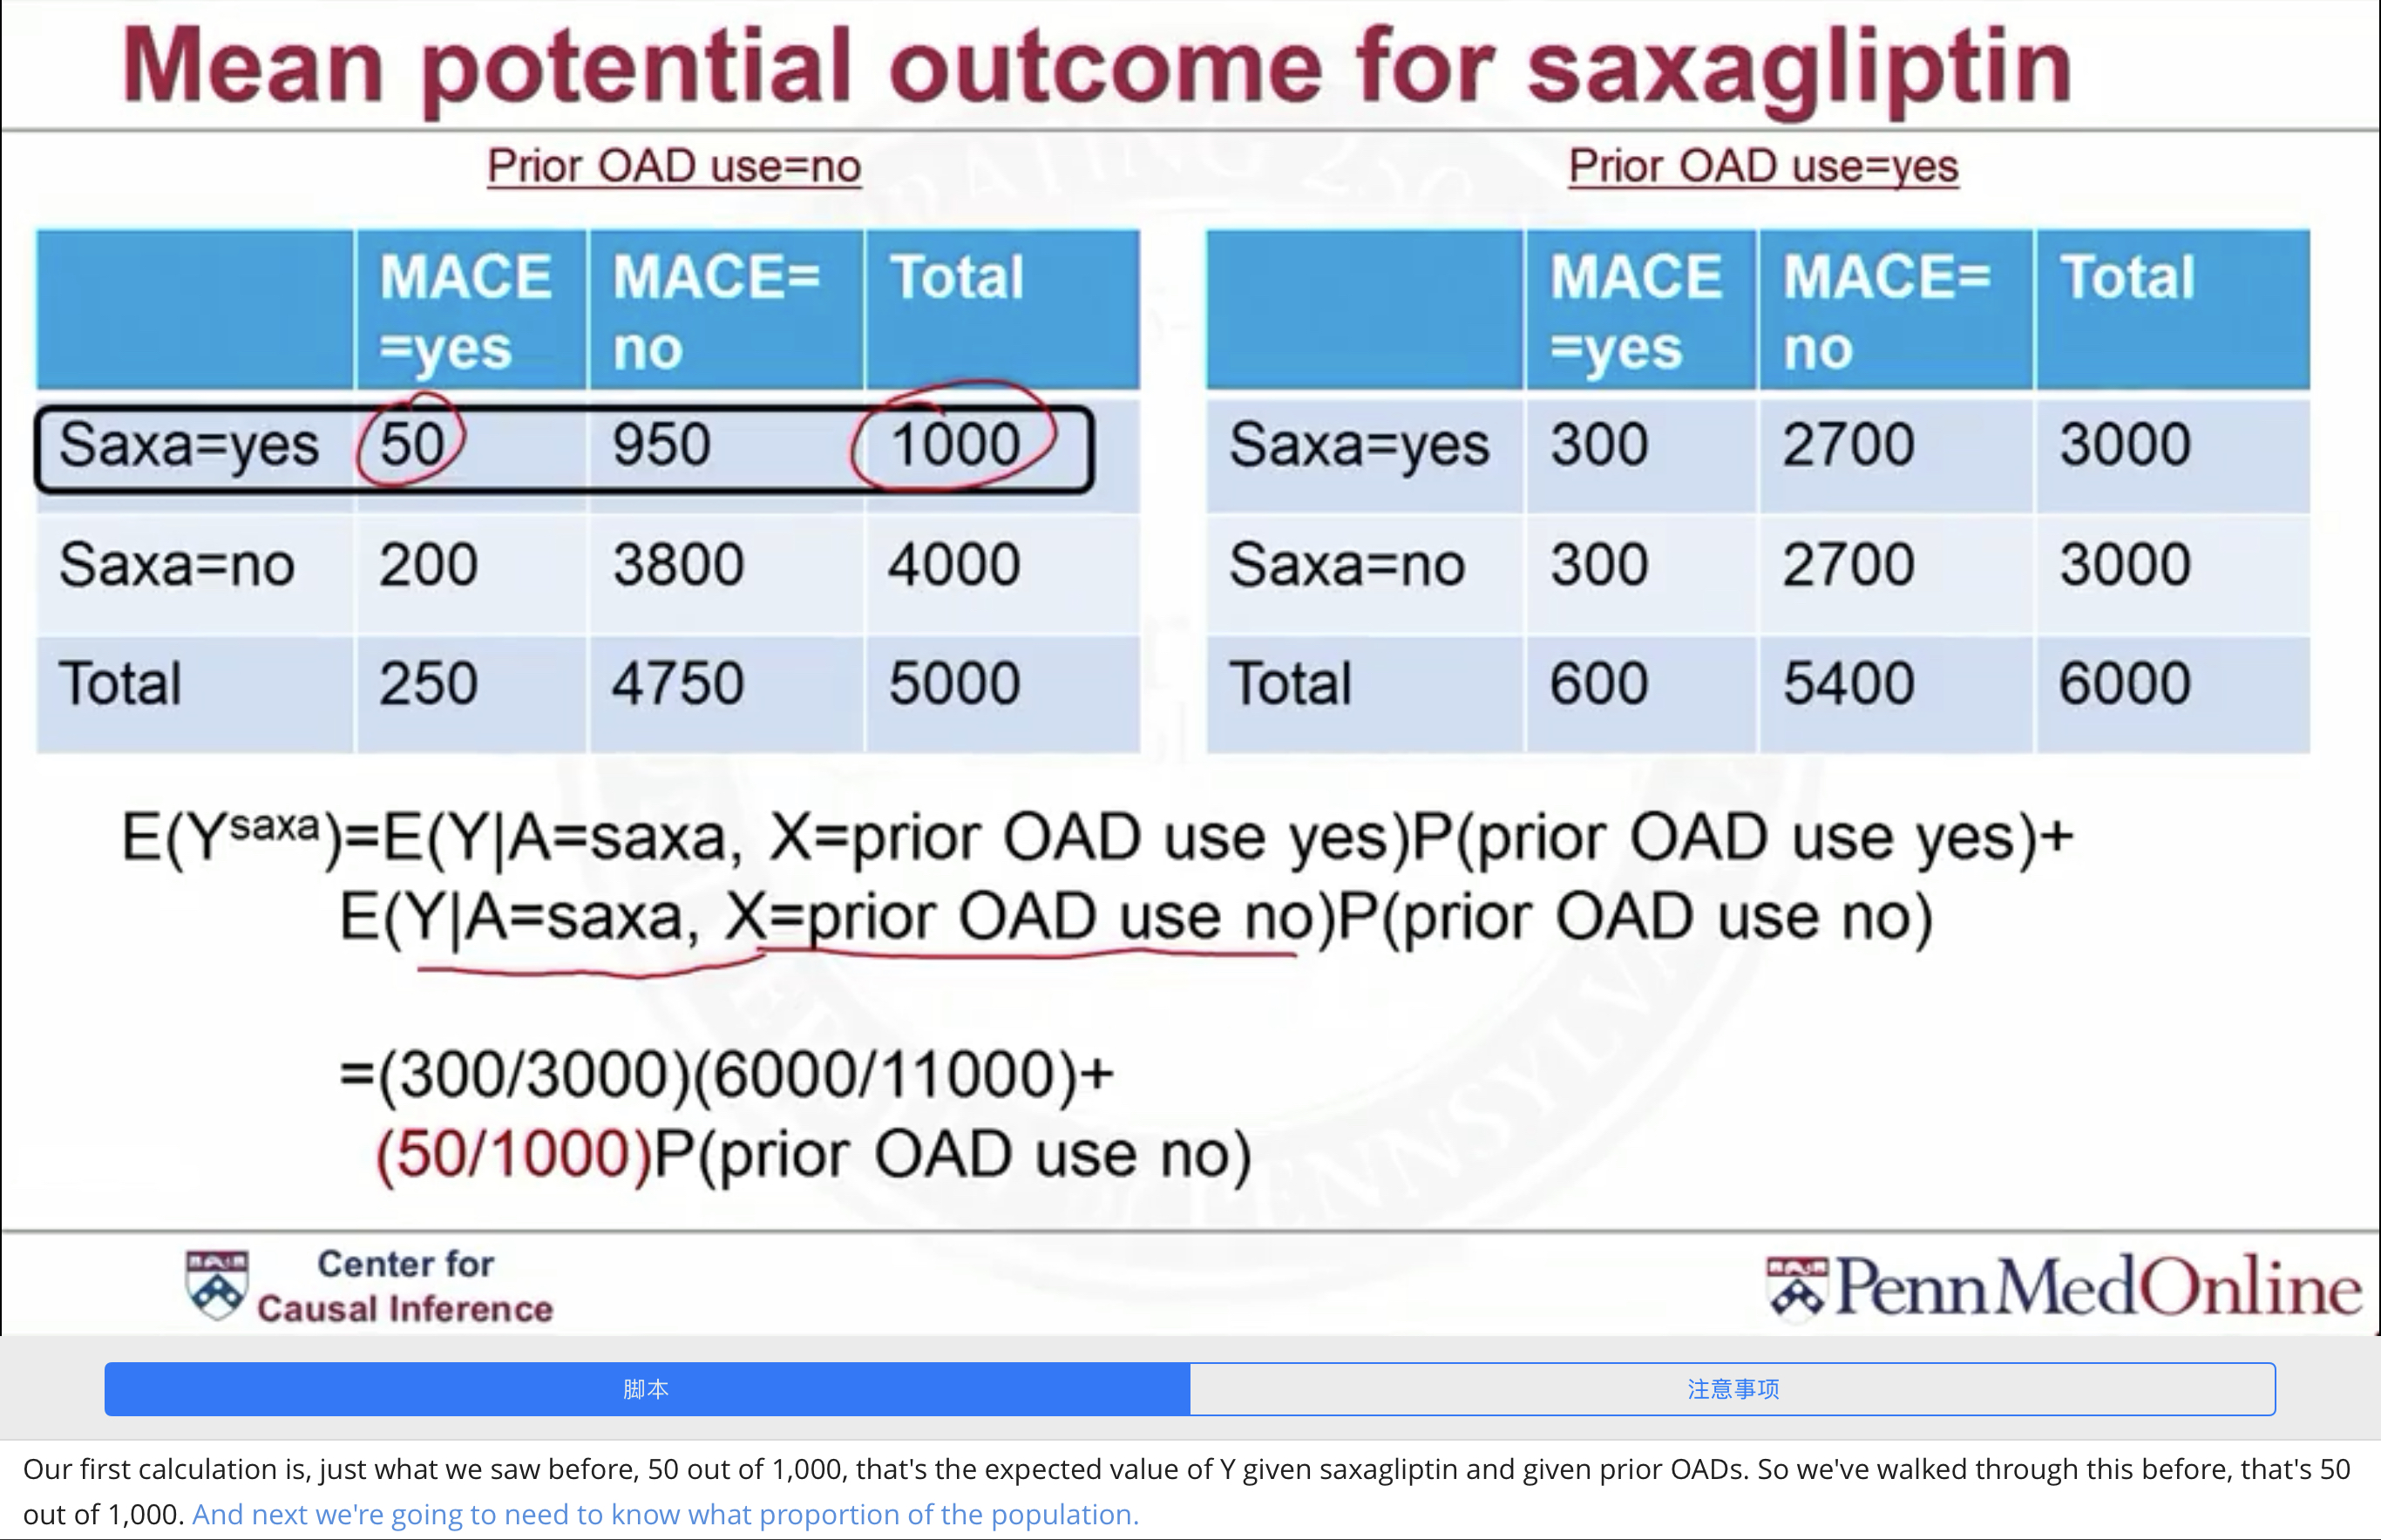
\includegraphics[width=0.8\textwidth]{figure/meansaxa.jpg}
	   \caption{Mean potential outcome for saxa}   
       \label{meansaxa}
       \end{figure}

	 \begin{figure}[htbp]
	 \setlength{\abovecaptionskip}{0pt}     %调整图片标题与图距离
	 \setlength{\belowcaptionskip}{10pt}
	 \vspace{-0cm}  %调整图片与上文的垂直距离
	 \setlength{\abovecaptionskip}{-0cm}   %调整图片标题与图距离
	 \setlength{\belowcaptionskip}{-0cm}   %调整图片标题与下文距离
	 \centering
     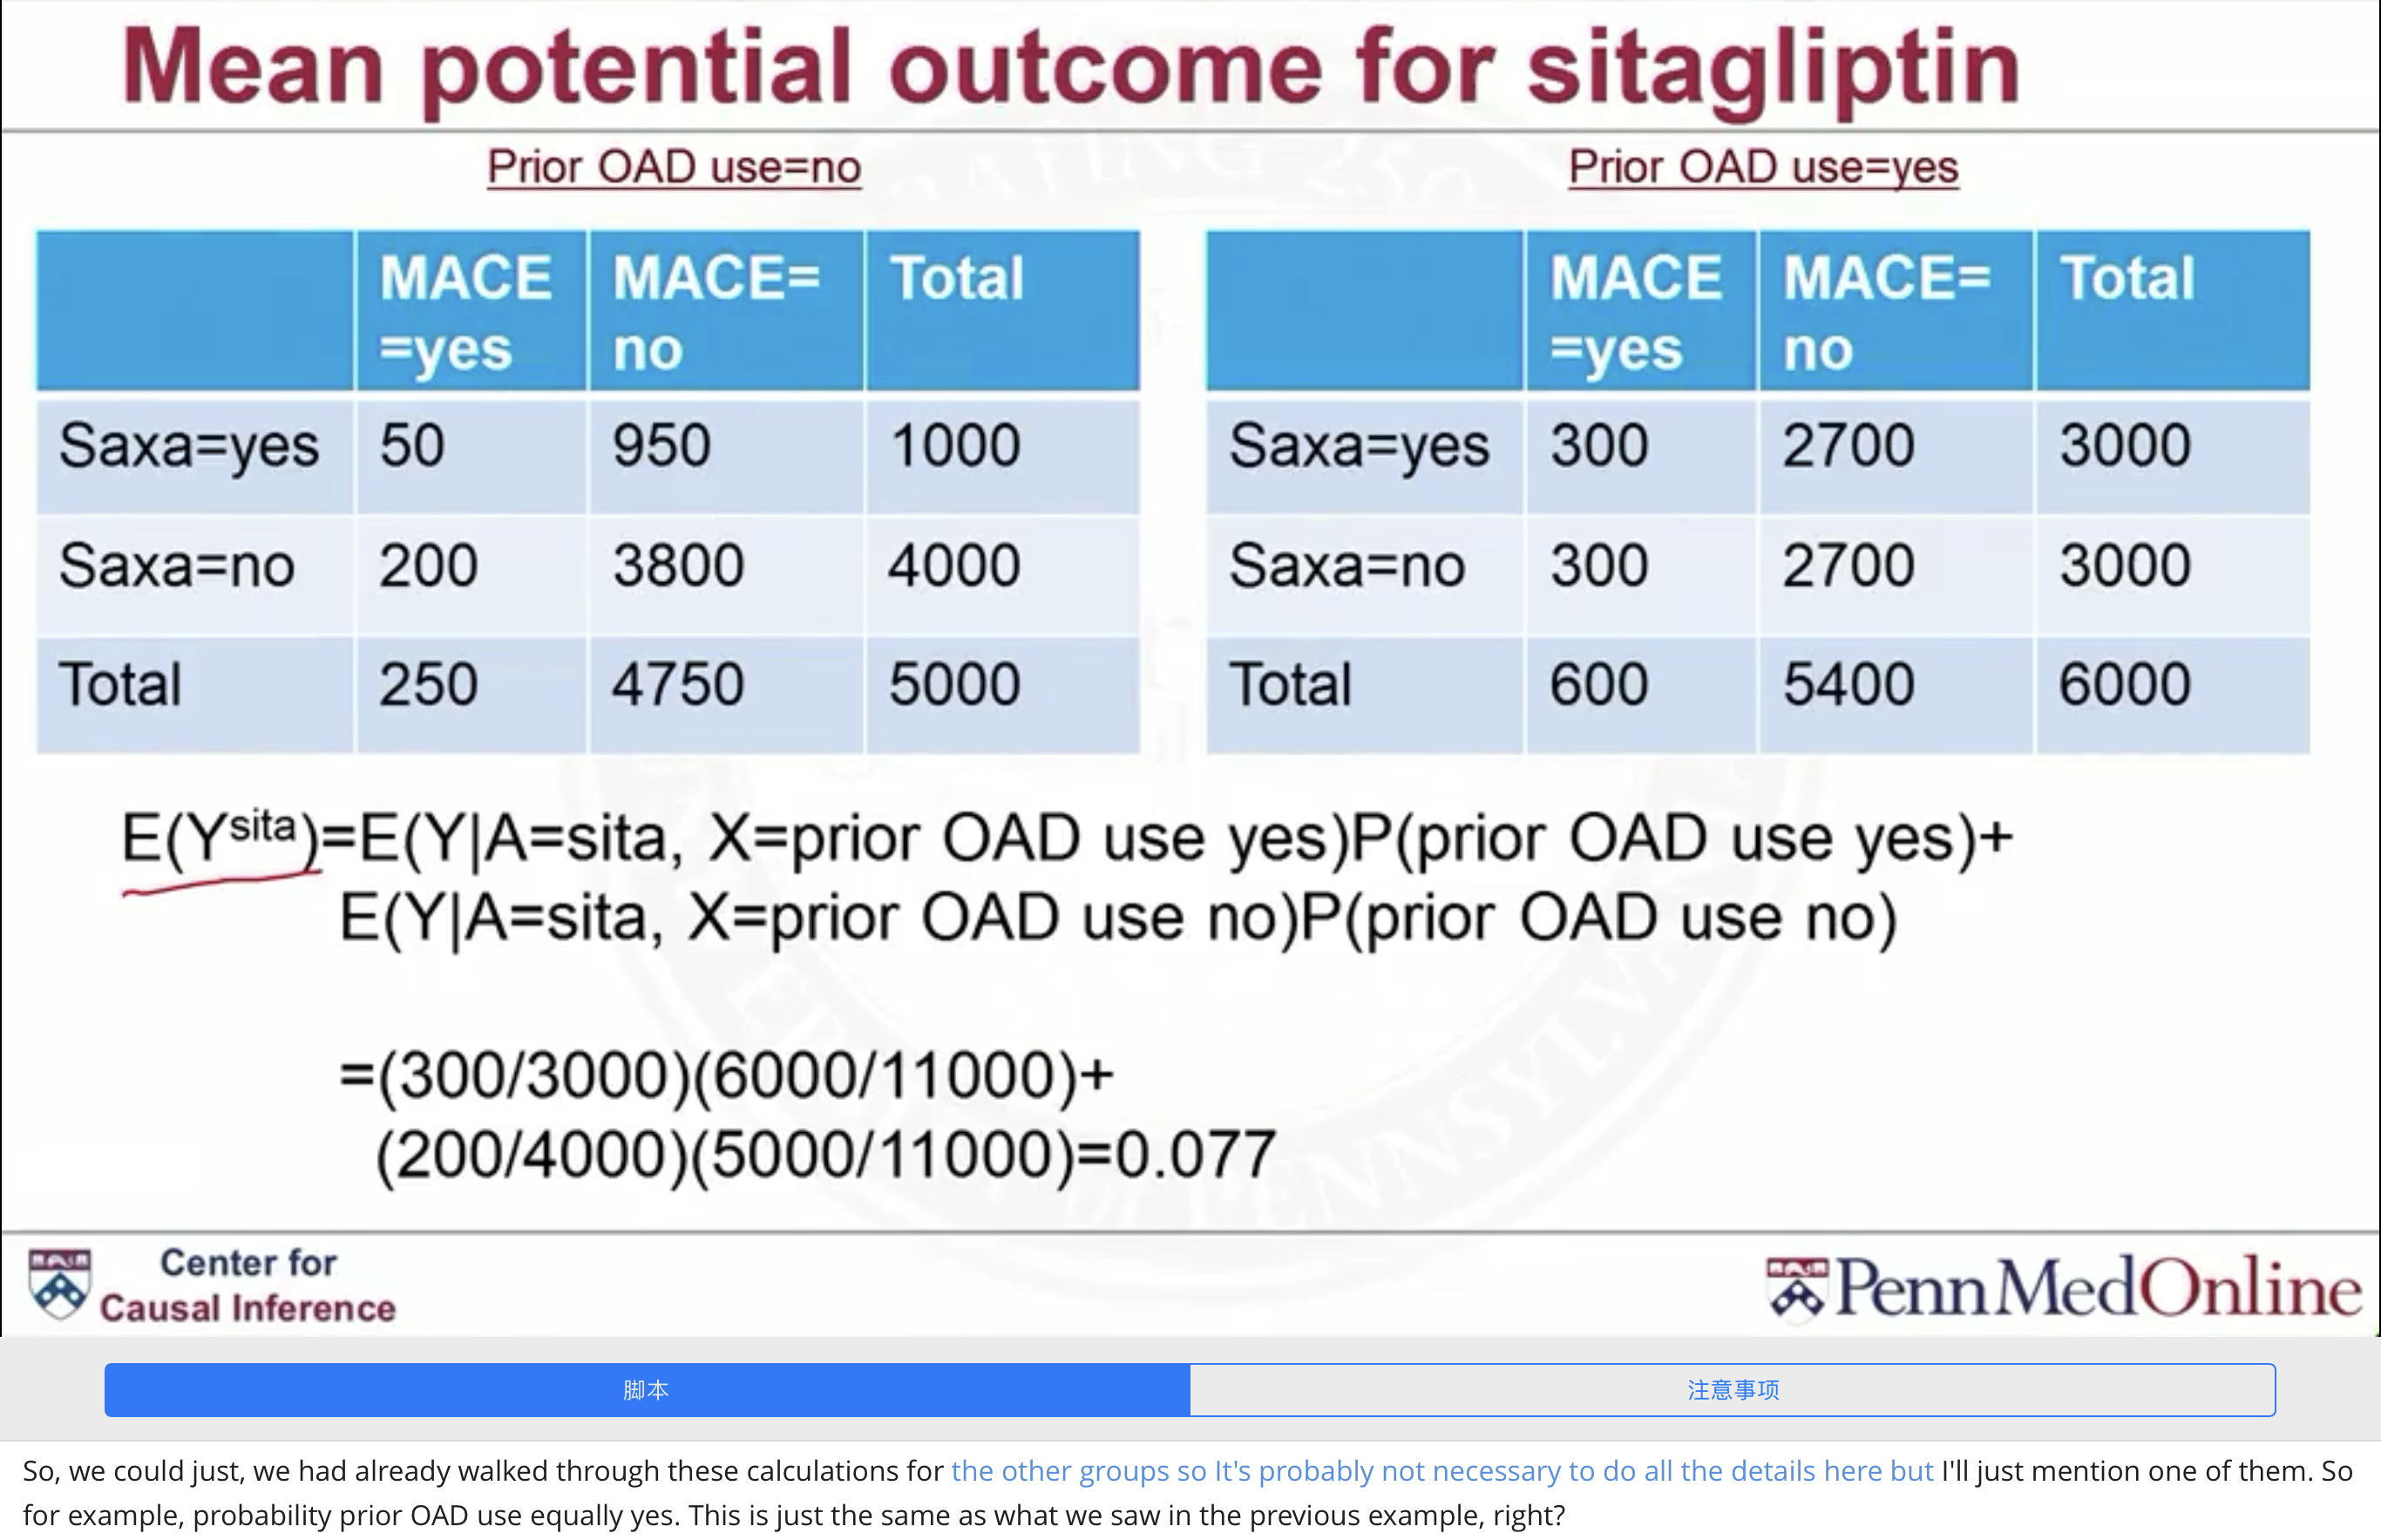
\includegraphics[width=0.8\textwidth]{figure/meansita.jpg} 
     \caption{Mean potential outcome for sita}
     \label{meansita}
     \end{figure}           
\subsection{Conclusion}
最后总结一下Stratification算法的缺陷:

\begin{figure}[h]
	\setlength{\abovecaptionskip}{0pt}     %调整图片标题与图距离
	\setlength{\belowcaptionskip}{10pt}
	\vspace{-0cm}  %调整图片与上文的垂直距离
	\setlength{\abovecaptionskip}{-0cm}   %调整图片标题与图距离
	%\setlength{\belowcaptionskip}{-0cm}   %调整图片标题与下文距离
	\centering
	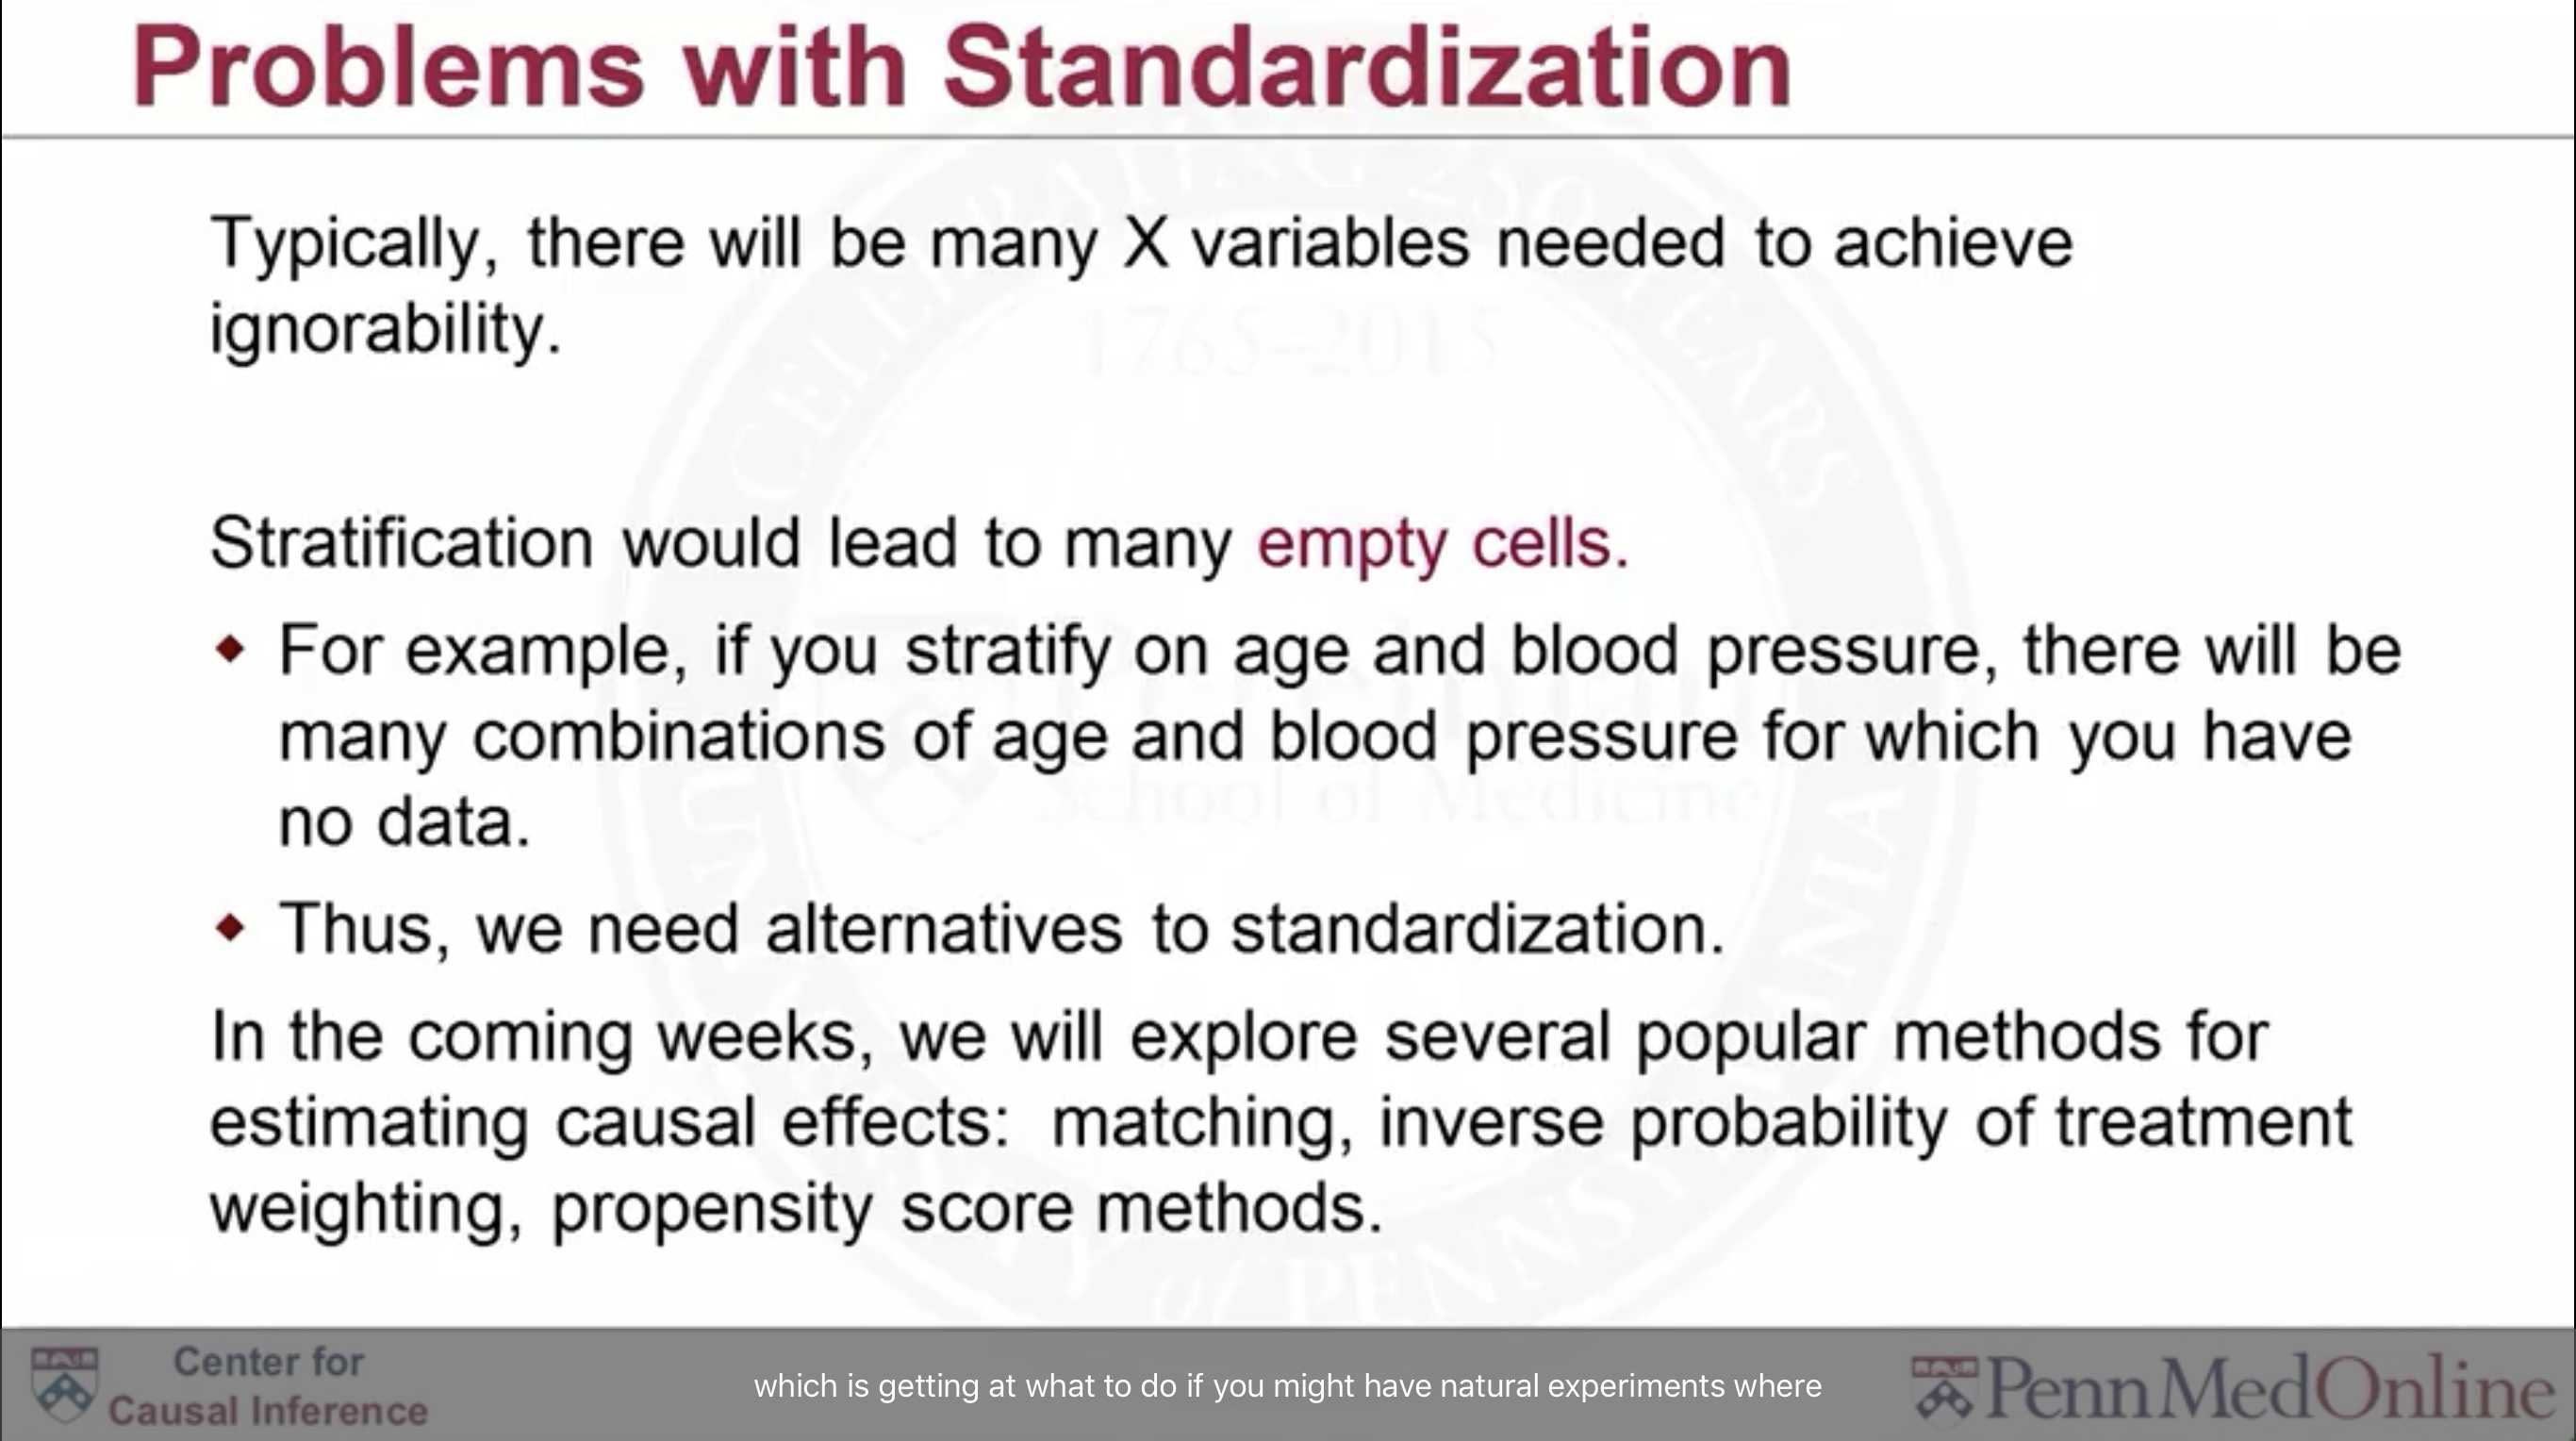
\includegraphics[width=0.8\textwidth]{figure/strtprm.jpg}
	\caption{Problems of Stratification}
	\label{strtprm}
\end{figure}

\newpage \section{Incident User and Active Comparator designs}
\noindent {\bfseries Outline:}\\
1. Two designs: Incident user design and active comparator designs.\\
2. Understand the basic idea of incident user design and what problem they help avoid.\\
3. Understand the basic idea of active comparator design and how they help to reduce confoundering.

\subsection{Cross-sectional look at treatments}
Suppose that we are interested in the causal effect of $A$ on the outcome $Y$. And we have a population of people, some of them are doing $A=1$, while some are not. Now suppose $A=$wheter regularly practicing yoga and $Y=$blood pressure. 

\paragraph{There are problems:} At any given time, some people regularly practice yoga while others not.
\begin{itemize}
	\item Those who do not might have in the past.
	\item Those who do might have bee practicing for a long time, or might be beginners.
	\item Why did some people quit and others continued? What if those that quit did so because yoga was not working?
\end{itemize}

This is a type of {\color{red} selection bias} that is very hard to control. 

\paragraph{{\color{red} If we are just looking at current treatment: yes or no, and ignore whole history of treatment, it will be difficult to control selection bias.}}

Here is an example about cross-sectional look
at treatments, like Fig.\ref{cstrt}.
\begin{figure}[htbp]
	\setlength{\abovecaptionskip}{0pt}     %调整图片标题与图距离
	\setlength{\belowcaptionskip}{10pt}
	\vspace{-0cm}  %调整图片与上文的垂直距离
	\setlength{\abovecaptionskip}{0pt}   %调整图片标题与图距离
	\setlength{\belowcaptionskip}{-5pt}   %调整图片标题与下文距离
	\centering
	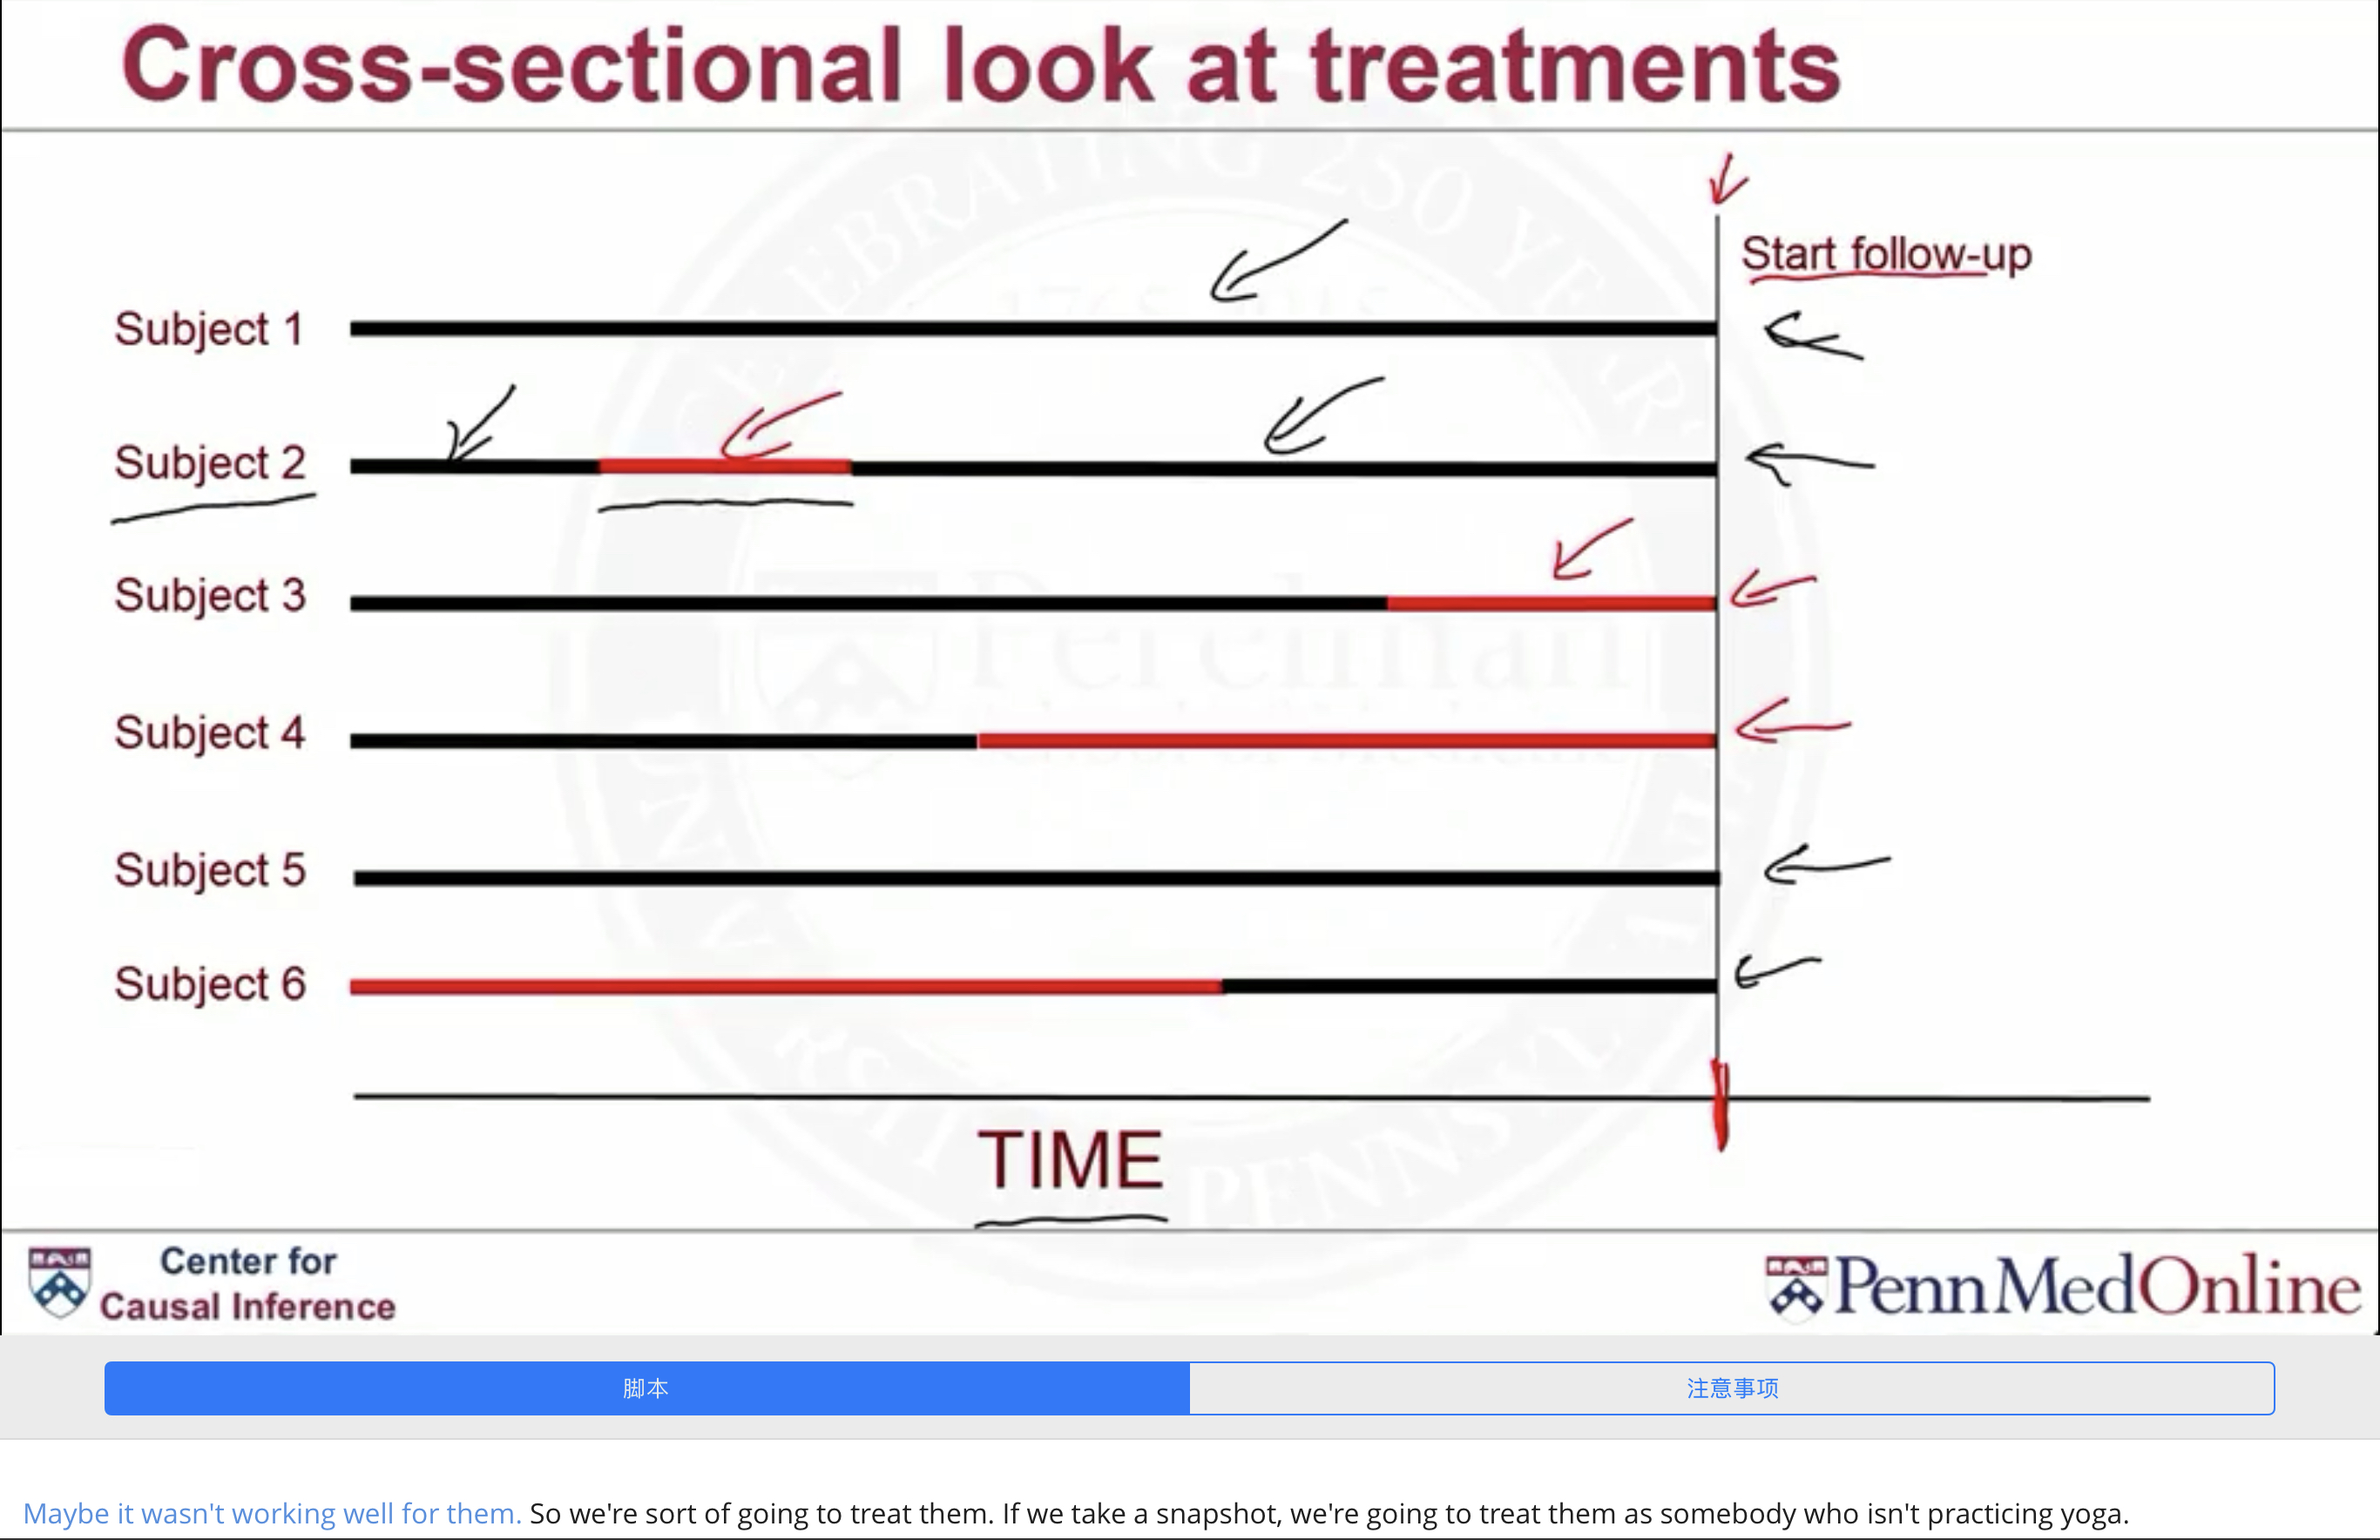
\includegraphics[width=0.8\textwidth]{figure/cstrt.jpg} 
	\caption{cross-sectional look at treatment}
	\label{cstrt}
\end{figure} 
Cross-sectional look 的问题在于:在观测节点之前,practicing yoga就已经产生了treatment effect,而这部分treatment effect又残留在新的观测数据中.

\subsection{New User design}
为解决上述问题,我们转而关注"people who newly initiaing treatment". 这种方法就是{\color{red} new user design}. 在new user design中,我们找到一些subjects刚好一致地从观测点开始treatment.

在这个过程中,关注的people发生了变换:
The treated people who is currently treated regardless of their treated history $\Longrightarrow$ new initiators. 

因此在某些程度上,我们关注的问题也发生了变化:
The causal effect of "practicing yoga" on "blood pressure" $\Longrightarrow$ the causal effect of "initiating practicing yoga" on "blood pressure". 

通过将问题转化成new user design,我们研究的causal effect就更加清楚,排除了上述的"selection bias"问题.
An example of new user design is given in Fig.\ref{nwud}:
\begin{figure}[htbp]
	\setlength{\abovecaptionskip}{0pt}     %调整图片标题与图距离
	\vspace{-0cm}  %调整图片与上文的垂直距离
	\setlength{\abovecaptionskip}{-0cm}   %调整图片标题与图距离
	\setlength{\belowcaptionskip}{0pt}   %调整图片标题与下文距离
	\centering
	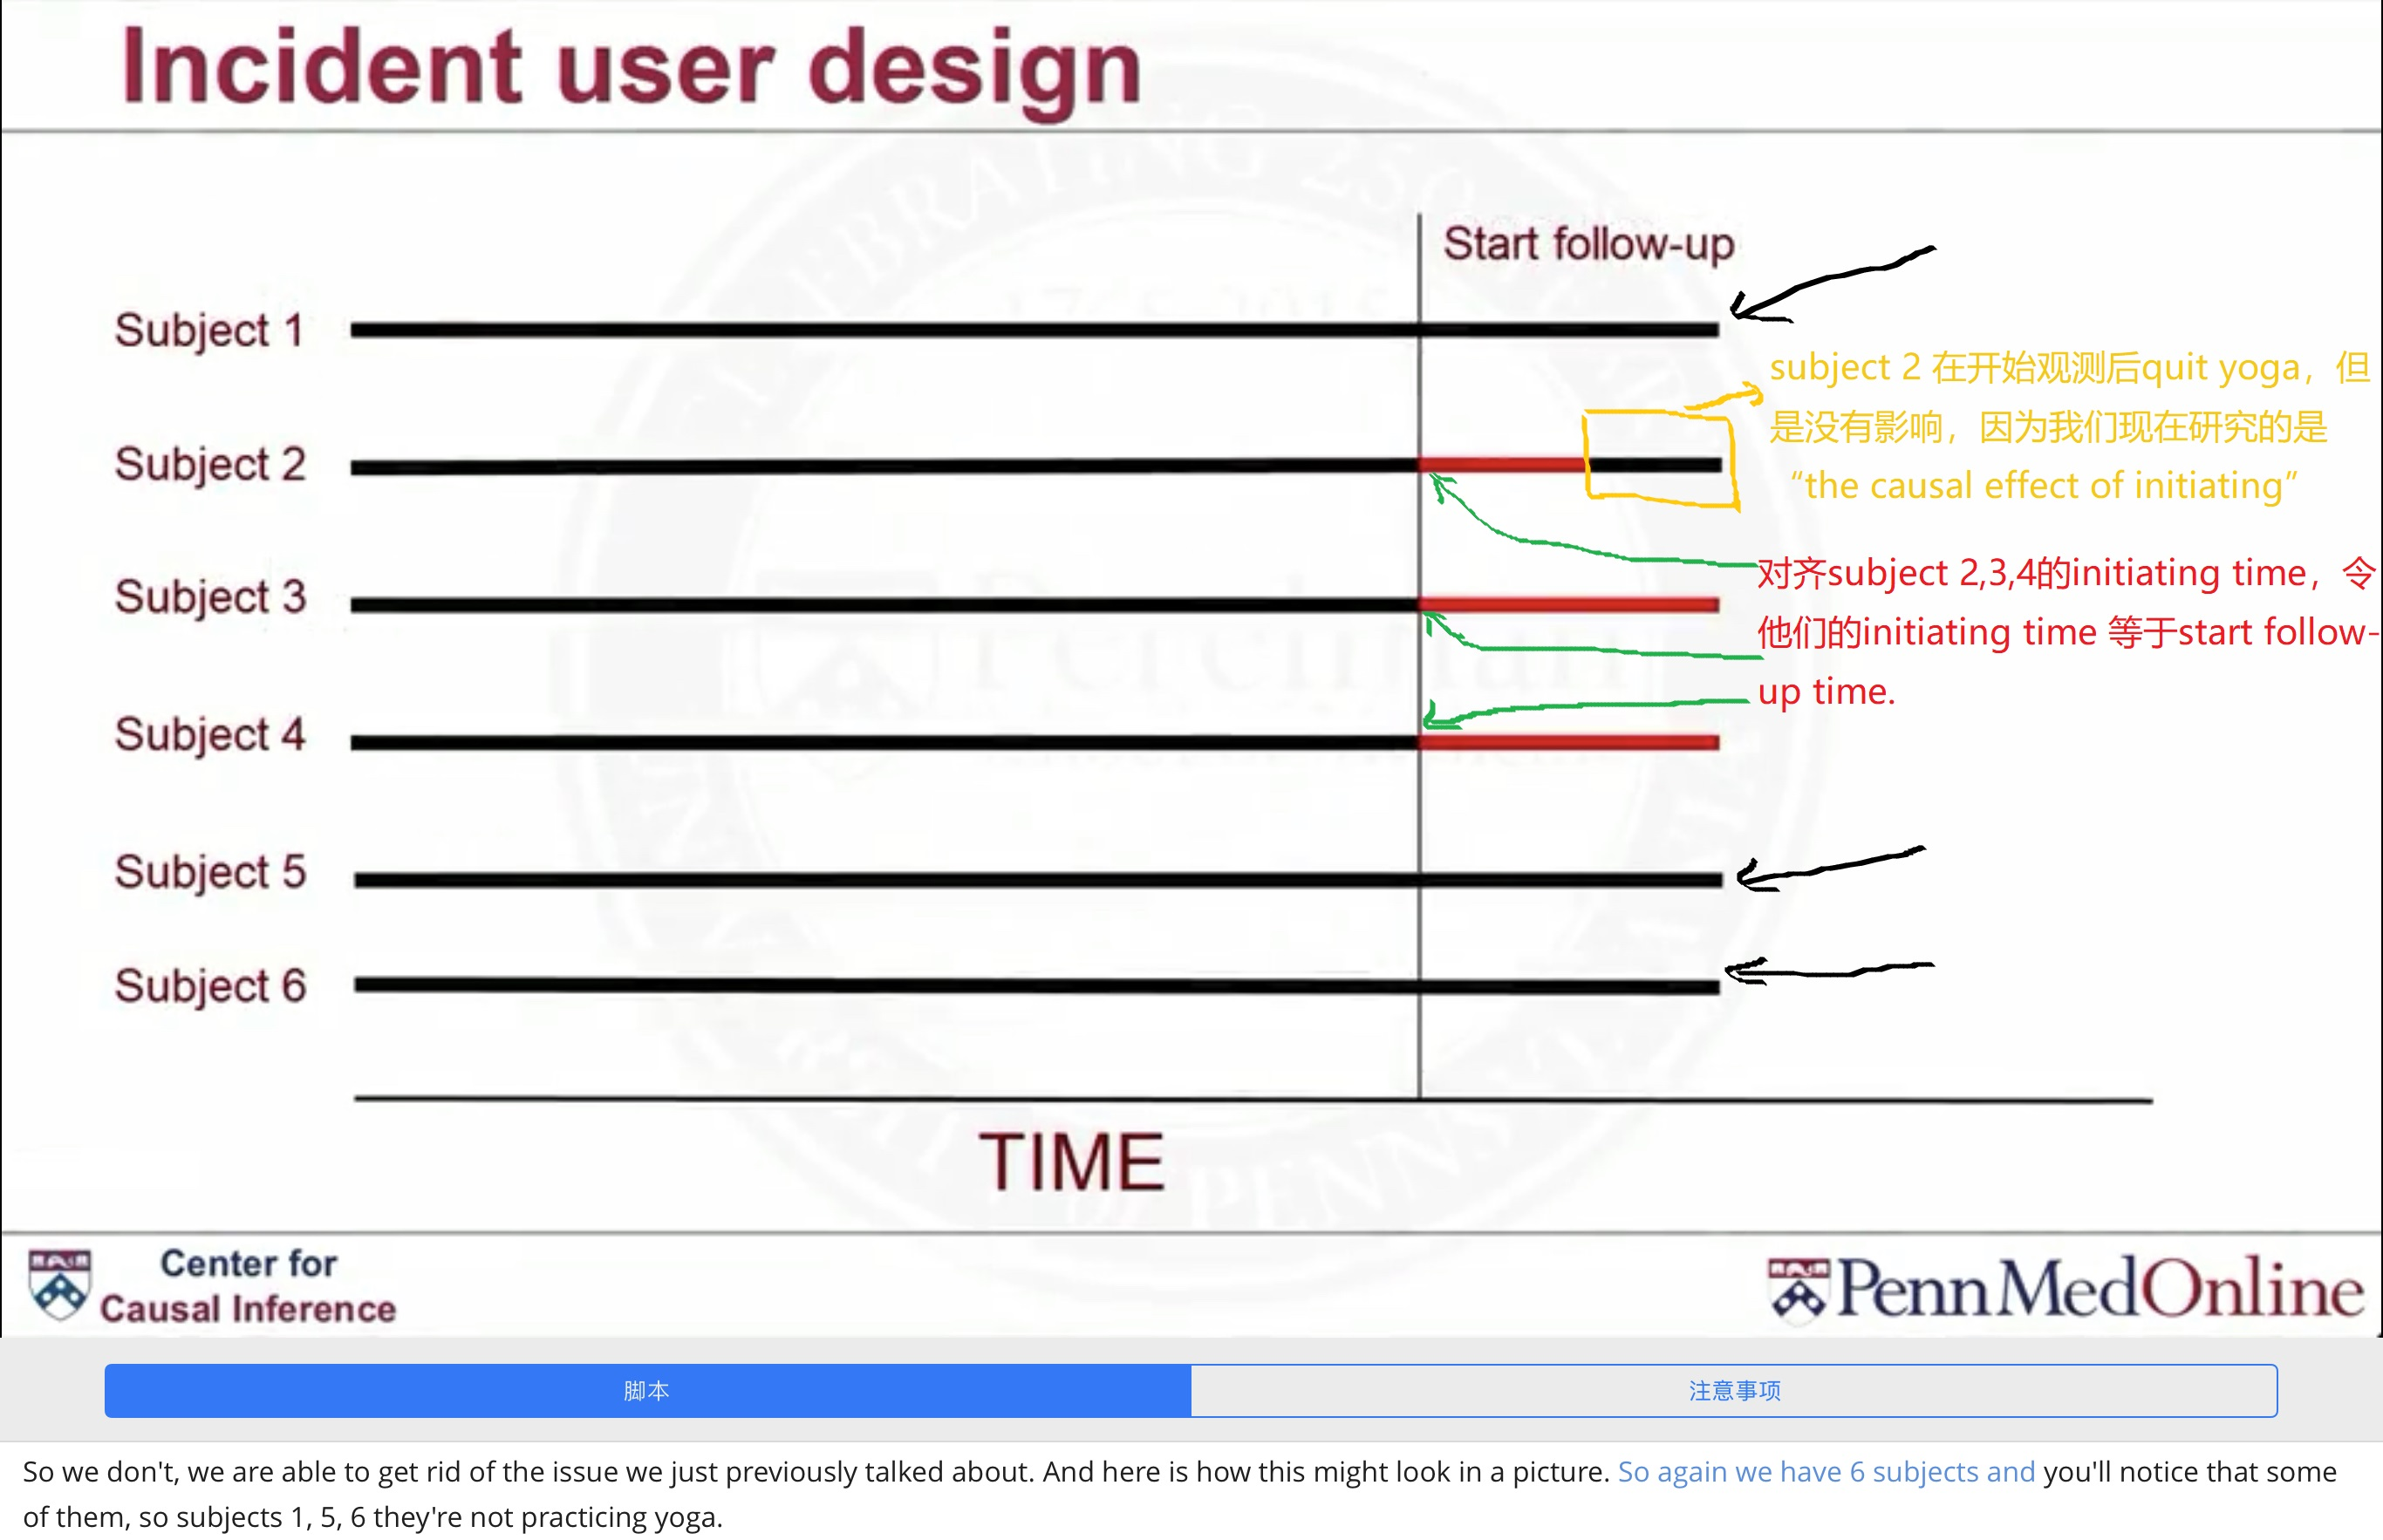
\includegraphics[width=0.8\textwidth]{figure/newud.jpg} 
	\caption{New user design}
	\label{newud}
\end{figure} 

\paragraph{The shortcome of incident user design:} 
\begin{enumerate}[label=\arabic*.]
	\item 我们已经注意到,incident user design将treated group限制在了{\color{red}"newly initiating treatment"的人群中,}因此我们只能考察{\color{red} “对于过去没有练过瑜伽的人,开始练习瑜伽后对血压的causal effect.”}
	\item {\bfseries It's hard to implement incident user design.} There's not going to be any period of time where people have no treatment.
    \item {\bfseries Untreated group的start follow-up问题.} 在New user design中,treated group中的subjects都有了明确的initiating time,我们可以设置start follow-up time,但是对于那些“从来没有接受过treatment”的人来说,start follow-up time却并不明确.
    \item {\bfseries Abvious difference between confounders of both groups.} 练习yoga的人和从不练习yoga的人在confounders上有着很大的不同,此时控制Confounders也是一个很大的问题.
\end{enumerate}

解决后面两个问题的一个方法是:再找一个treatment,与现有的treatment形成对比组. 这就是接下来要说的另一种design——active comparator design.

\subsection{Active Comparator Design}
如果比较两种treatment"initiate yoga"和"initiate Zumba"对于"blood pressure"的影响,问题就变成了"active comparator design".
Fig.\ref{acd}给出了两个具体的例子.
\begin{figure}[htbp]
	\setlength{\abovecaptionskip}{0pt}     %调整图片标题与图距离
	\setlength{\belowcaptionskip}{10pt}
	\vspace{-0cm}  %调整图片与上文的垂直距离
	\setlength{\abovecaptionskip}{-0cm}   %调整图片标题与图距离
	\setlength{\belowcaptionskip}{-0cm}   %调整图片标题与下文距离
	\centering
	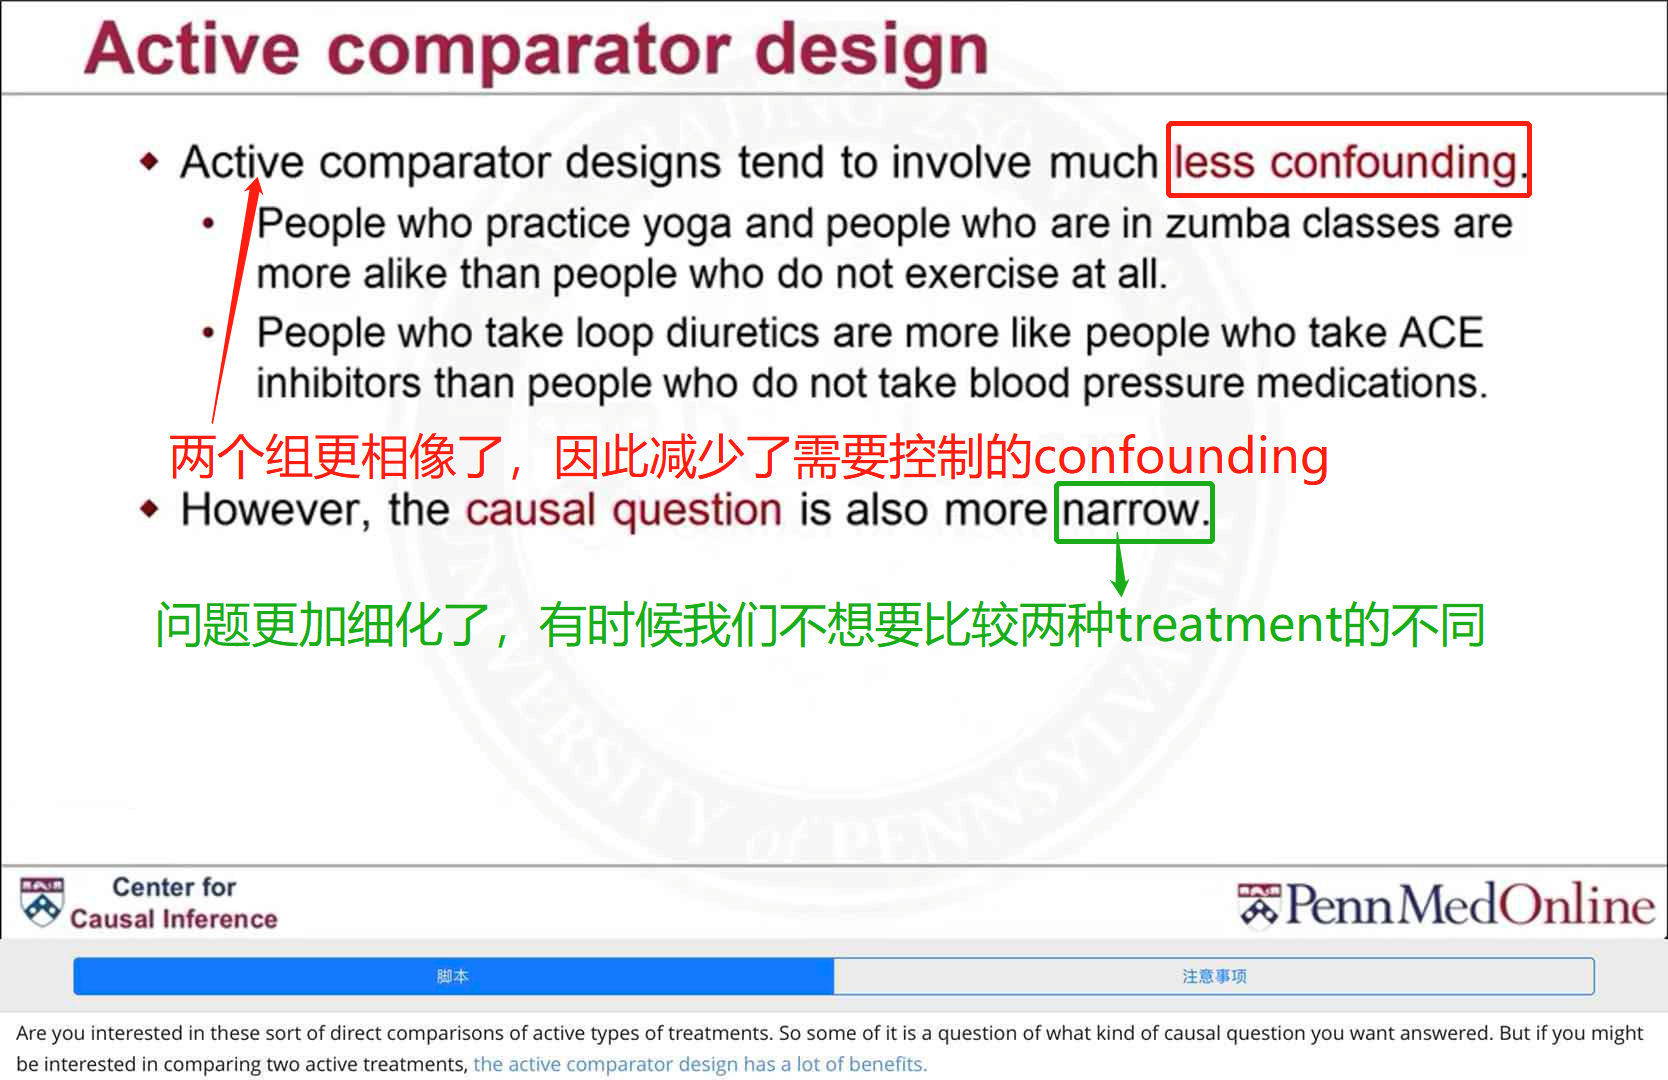
\includegraphics[width=0.8\textwidth]{figure/acd.png} 
	\caption{Active comparator design}
	\label{acd}
\end{figure} 

假设我们收集到了6个样本,如Fig.\ref{exacd}所示.
\begin{figure}[htbp]
	\setlength{\abovecaptionskip}{0pt}     %调整图片标题与图距离
	\setlength{\belowcaptionskip}{10pt}
	\vspace{-0cm}  %调整图片与上文的垂直距离
	\setlength{\abovecaptionskip}{-0cm}   %调整图片标题与图距离
	\setlength{\belowcaptionskip}{-0cm}   %调整图片标题与下文距离
	\centering
	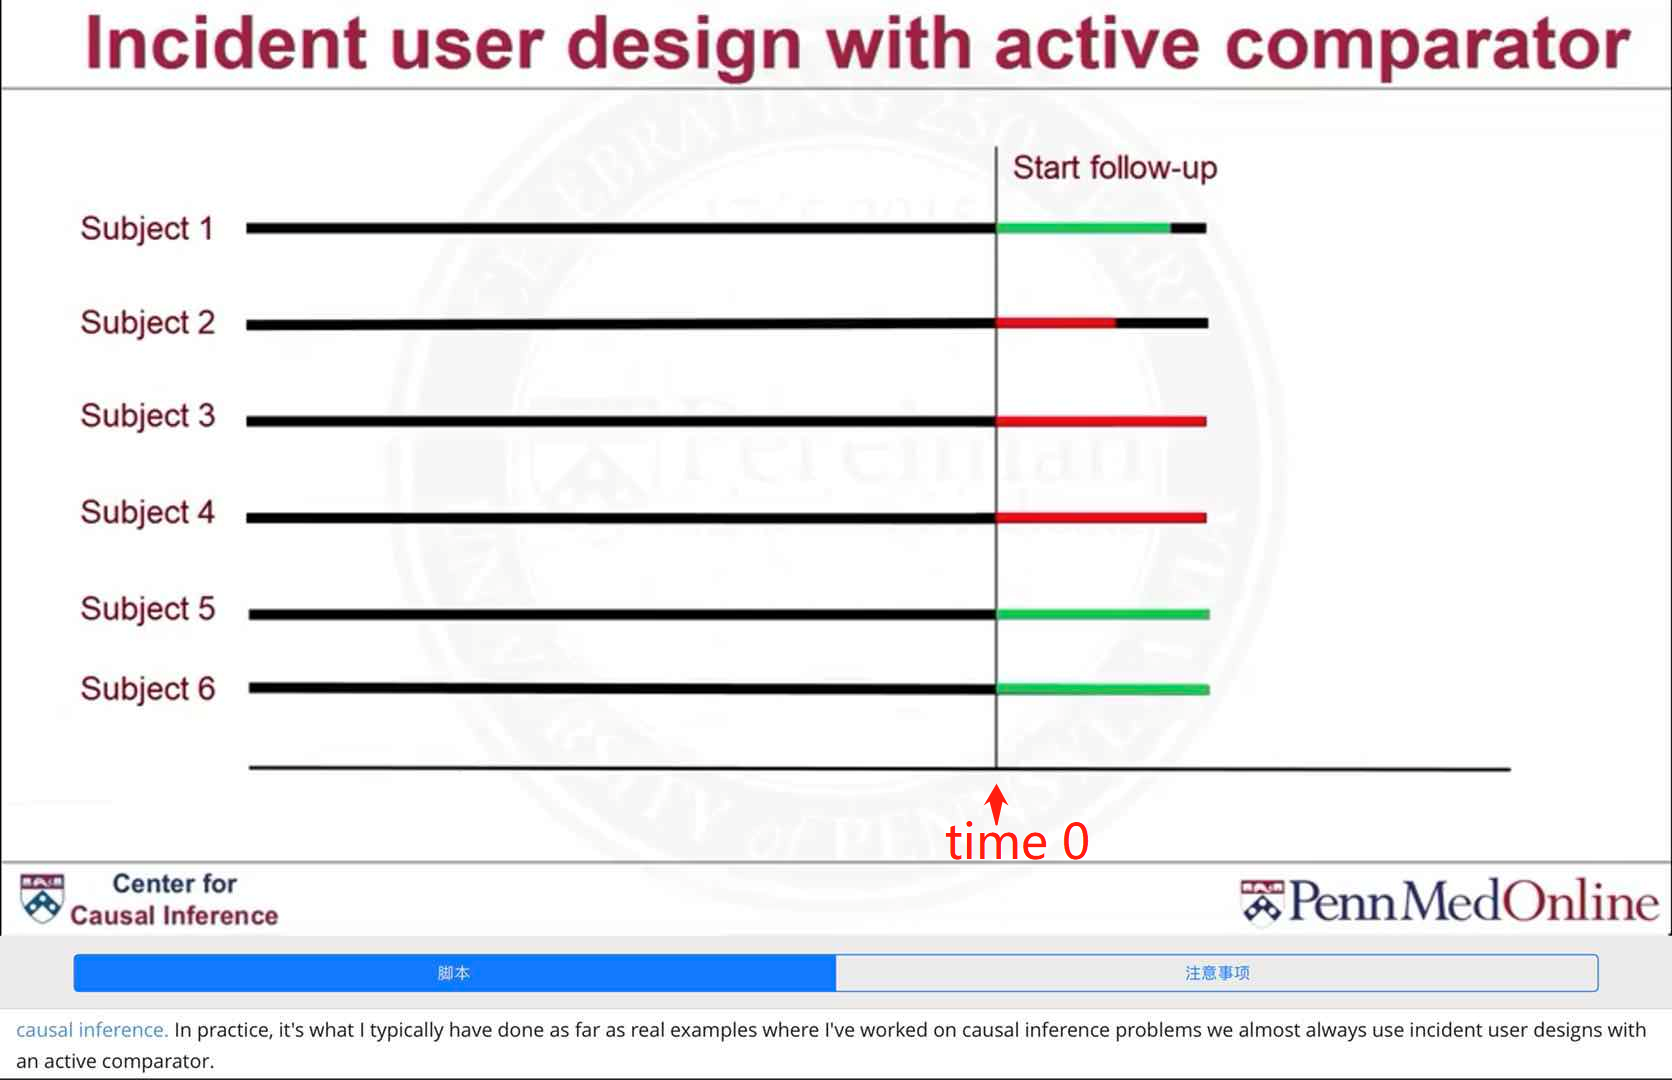
\includegraphics[width=0.8\textwidth]{figure/exacd.png} 
	\caption{New user design with active comparator}
	\label{exacd}
\end{figure} 

We note that the confounders that we can control for would be variables that were measured prior to time 0.

\paragraph{Issues of active comparator design.} 
\begin{enumerate}[label=\arabic*.]
	\item We are not interested in comparing to some active treatment. The causal question is too narrow.
	\item 与new user design的问题相同. There's not going to be any period of time where people have no treatment.
\end{enumerate}

\subsection{Conclusion}
最后总结一下这两种design存在的问题:
\begin{figure}[htbp]
	\setlength{\abovecaptionskip}{0pt}     %调整图片标题与图距离
	\setlength{\belowcaptionskip}{10pt}
	\vspace{-0cm}  %调整图片与上文的垂直距离
	\setlength{\abovecaptionskip}{-0cm}   %调整图片标题与图距离
	\setlength{\belowcaptionskip}{-0cm}   %调整图片标题与下文距离
	\centering
	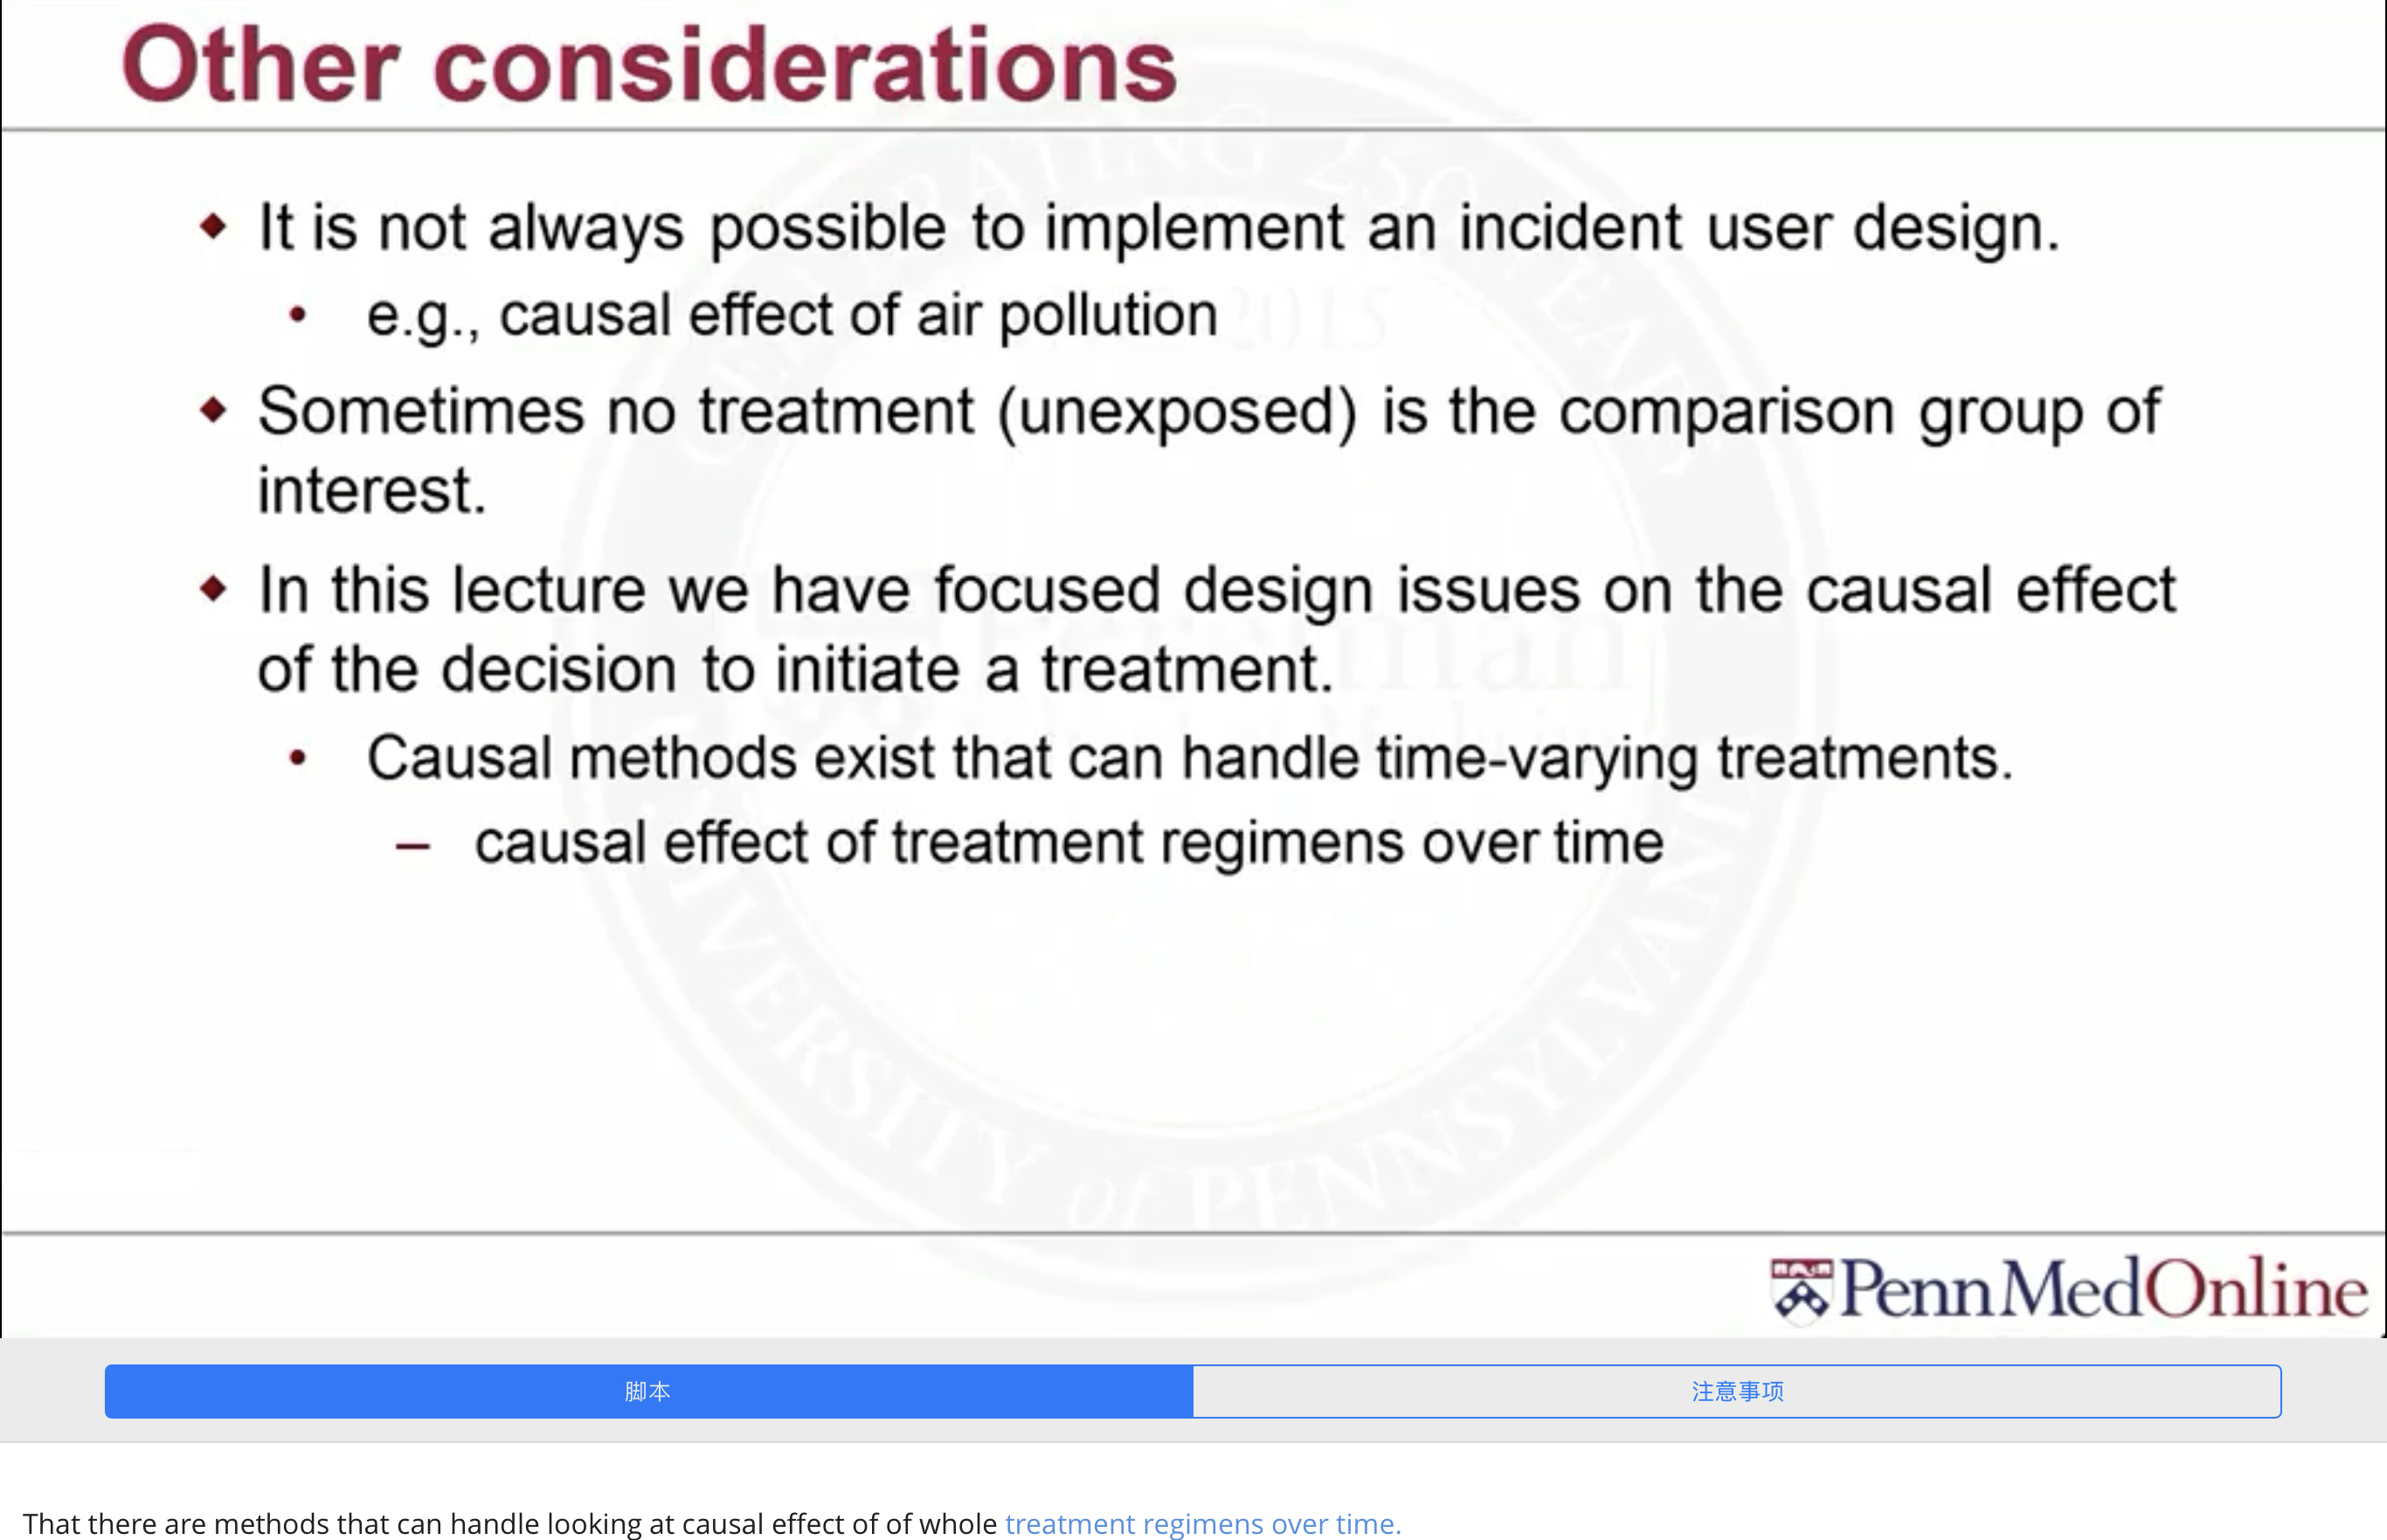
\includegraphics[width=0.8\textwidth]{figure/othercon.jpg} 
	\caption{Conclusion of the two designs}
	\label{othercon}
\end{figure} 

需要说明的是{\color{red}there are causal methods that can handle time variant treatments where we might be looking at the causal effects of treatments over time.}



